\documentclass{vkr}
\usepackage[english, russian]{babel} % переносы
\usepackage{graphicx} % для вставки картинок
\graphicspath{{images/}} % путь к изображениям
\usepackage[hidelinks]{hyperref}
\usepackage{float} % определяет метод H для рисунка с переносом на следующую страницу, ели не помещается
\usepackage{pdflscape}
\addto{\captionsrussian}{\renewcommand{\refname}{СПИСОК ИСПОЛЬЗОВАННЫХ ИСТОЧНИКОВ}}
\usepackage{xltabular} % для вставки таблиц
\usepackage{makecell}
\renewcommand\theadfont{} % шрифт в /thead
\usepackage{array} % для определения новых типов столбцов таблиц
\newcolumntype{T}{>{\centering\arraybackslash}X} % новый тип столбца T - автоматическая ширина столбца с выравниванием по центру
\newcolumntype{R}{>{\raggedleft\arraybackslash}X} % новый тип столбца R - автоматическая ширина столбца с выравниванием по правому краю
\newcolumntype{C}[1]{>{\centering\let\newline\\\arraybackslash\hspace{0pt}}m{#1}} % новый тип столбца C - фиксированная ширина столбца с выравниванием по центру
\newcolumntype{r}[1]{>{\raggedleft\arraybackslash}p{#1}} % новый тип столбца r - фиксированная ширина столбца с выравниванием по правому краю
\newcommand{\centrow}{\centering\arraybackslash} % командой \centrow можно центрировать одну ячейку (заголовок) в столбце типа X или p, оставив в оcтальных ячейках другой тип выравнивания
\newcommand{\finishhead}{\endhead\hline\endlastfoot}
\newcommand{\continuecaption}[1]{\captionsetup{labelformat=empty} \caption[]{#1}\\ \hline }
\usepackage{etoolbox}
\AtBeginEnvironment{xltabular}{\refstepcounter{tablecnt}} % подсчет таблиц xltabular, обычные таблицы подсчитываются в классе

\usepackage[tableposition=top]{caption} % подпись таблицы вверху
\captionsetup{strut=off}
\setlength{\intextsep}{0pt} % Vertical space above & below [h] floats
\setlength{\textfloatsep}{0pt} % Vertical space below (above) [t] ([b]) floats
\DeclareCaptionLabelFormat{gostfigure}{Рисунок #2} %подпись рисунка
\DeclareCaptionLabelFormat{gosttable}{Таблица #2} %подпись таблицы
\DeclareCaptionLabelSeparator{gost}{~--~} %разделитель в рисунках и таблицах
\captionsetup{labelsep=gost}
\captionsetup[figure]{aboveskip=10pt,belowskip=4mm,justification=centering,labelformat=gostfigure} % настройка подписи рисунка
\captionsetup[table]{font={stretch=1.41},skip=0pt,belowskip=0pt,aboveskip=8.5pt,singlelinecheck=off,labelformat=gosttable} % настройка подписи таблицы

\setlength{\LTpre}{8mm} % отступ сверху таблицы
\setlength{\LTpost}{6mm} % отступ снизу таблицы

\usepackage{enumitem}
\setlist{nolistsep,wide=\parindent,itemindent=*} % отступы вокруг списков, выравнивание с учетом разделителя

\usepackage{color} %% это для отображения цвета в коде
\usepackage{listings} %% листинги кода
\setmonofont[Scale=0.7]{Verdana} % моноширный шрифт для листинга

\definecolor{codegreen}{rgb}{0,0.6,0}
\definecolor{codegray}{rgb}{0.5,0.5,0.5}
\definecolor{codepurple}{rgb}{0.58,0,0.82}

\lstset{ %
language=C,                 % выбор языка для подсветки (здесь это С)
numbers=left,               % где поставить нумерацию строк (слева\справа)
numberstyle=\tiny,           % размер шрифта для номеров строк
stepnumber=1,                   % размер шага между двумя номерами строк
numbersep=5pt,                % как далеко отстоят номера строк от подсвечиваемого кода
commentstyle=\color{codegreen},
keywordstyle=\color{magenta},
numberstyle=\tiny\color{codegray},
stringstyle=\color{codepurple},
basicstyle=\linespread{0.95}\ttfamily,
backgroundcolor=\color{white}, % цвет фона подсветки - используем \usepackage{color}
showspaces=false,            % показывать или нет пробелы специальными отступами
showstringspaces=false,      % показывать или нет пробелы в строках
showtabs=false,             % показывать или нет табуляцию в строках
frame=single,              % рисовать рамку вокруг кода
tabsize=2,                 % размер табуляции по умолчанию равен 2 пробелам
captionpos=t,              % позиция заголовка вверху [t] или внизу [b] 
breaklines=true,           % автоматически переносить строки (да\нет)
breakatwhitespace=false, % переносить строки только если есть пробел
escapeinside={\%*}{*)}   % если нужно добавить комментарии в коде
}

\makeatletter % чтобы допускались русские комментарии в листингах
\lst@InputCatcodes
\def\lst@DefEC{%
 \lst@CCECUse \lst@ProcessLetter
  ^^80^^81^^82^^83^^84^^85^^86^^87^^88^^89^^8a^^8b^^8c^^8d^^8e^^8f%
  ^^90^^91^^92^^93^^94^^95^^96^^97^^98^^99^^9a^^9b^^9c^^9d^^9e^^9f%
  ^^a0^^a1^^a2^^a3^^a4^^a5^^a6^^a7^^a8^^a9^^aa^^ab^^ac^^ad^^ae^^af%
  ^^b0^^b1^^b2^^b3^^b4^^b5^^b6^^b7^^b8^^b9^^ba^^bb^^bc^^bd^^be^^bf%
  ^^c0^^c1^^c2^^c3^^c4^^c5^^c6^^c7^^c8^^c9^^ca^^cb^^cc^^cd^^ce^^cf%
  ^^d0^^d1^^d2^^d3^^d4^^d5^^d6^^d7^^d8^^d9^^da^^db^^dc^^dd^^de^^df%
  ^^e0^^e1^^e2^^e3^^e4^^e5^^e6^^e7^^e8^^e9^^ea^^eb^^ec^^ed^^ee^^ef%
  ^^f0^^f1^^f2^^f3^^f4^^f5^^f6^^f7^^f8^^f9^^fa^^fb^^fc^^fd^^fe^^ff%
  ^^^^20ac^^^^0153^^^^0152%
  % Basic Cyrillic alphabet coverage
  ^^^^0410^^^^0411^^^^0412^^^^0413^^^^0414^^^^0415^^^^0416^^^^0417%
  ^^^^0418^^^^0419^^^^041a^^^^041b^^^^041c^^^^041d^^^^041e^^^^041f%
  ^^^^0420^^^^0421^^^^0422^^^^0423^^^^0424^^^^0425^^^^0426^^^^0427%
  ^^^^0428^^^^0429^^^^042a^^^^042b^^^^042c^^^^042d^^^^042e^^^^042f%
  ^^^^0430^^^^0431^^^^0432^^^^0433^^^^0434^^^^0435^^^^0436^^^^0437%
  ^^^^0438^^^^0439^^^^043a^^^^043b^^^^043c^^^^043d^^^^043e^^^^043f%
  ^^^^0440^^^^0441^^^^0442^^^^0443^^^^0444^^^^0445^^^^0446^^^^0447%
  ^^^^0448^^^^0449^^^^044a^^^^044b^^^^044c^^^^044d^^^^044e^^^^044f%
  ^^^^0401^^^^0451%
  %%%
  ^^00}
\lst@RestoreCatcodes
\makeatother


% Режим шаблона (должен быть включен один из трех)
%\ВКРtrue
\Практикаtrue
%\Курсоваяtrue

\newcommand{\Дисциплина}{<<Проектирование и архитектура программных систем>>} % для курсовой
\newcommand{\КодСпециальности}{09.03.04} % Курсовая
\newcommand{\Специальность}{Программная инженерия} % Курсовая
\newcommand{\Тема}{Программная реализация системы управления проектами} % ВКР Курсовая
% \newcommand{\ТемаВтораяСтрока}{}
\newcommand{\ГдеПроводитсяПрактика}{ООО "МЦОБ. Онлайн-сервисы"}
\newcommand{\РуководительПрактПредпр}{Куркина А. В.} % для практики
\newcommand{\ДолжнРуководительПрактПредпр}{директор} % для практики
\newcommand{\РуководительПрактУнивер}{Чаплыгин А. А.} % для практики
\newcommand{\ДолжнРуководительПрактУнивер}{к.т.н. доцент} % для практики
\newcommand{\Автор}{А. Ю. Геворкян}
\newcommand{\АвторРод}{Геворкян А. Ю.}
\newcommand{\АвторПолностьюРод}{Геворкян Арнольда Юрьевича} % для практики
\newcommand{\Шифр}{21-06-0040}
\newcommand{\Курс}{4 } % для практики
\newcommand{\Группа}{ПО-11б}
\newcommand{\Руководитель}{Р. А. Томакова} % для ВКР и курсовой
\newcommand{\Нормоконтроль}{А. А. Чаплыгин} % для ВКР
\newcommand{\ЗавКаф}{А. В. Малышев} % для ВКР
\newcommand{\ДатаПриказа}{«07» апреля 2023~г.} % для ВКР
\newcommand{\НомерПриказа}{1505-с} % для ВКР
\newcommand{\СрокПредоставления}{«13» июня 2023~г.} % для ВКР, курсового

\begin{document}
\maketitle
\ifПрактика{}\else{
   \newpage
\begin{center}
\large\textbf{Минобрнауки России}

\large\textbf{Юго-Западный государственный университет}
\vskip 1em
\normalsize{Кафедра программной инженерии}
\vskip 1em
\ifВКР{
        \begin{flushright}
        \begin{tabular}{p{.4\textwidth}}
        \centrow УТВЕРЖДАЮ: \\
        \centrow Заведующий кафедрой \\
        \hrulefill \\
        \setarstrut{\footnotesize}
        \centrow\footnotesize{(подпись, инициалы, фамилия)}\\
        \restorearstrut
        «\underline{\hspace{1cm}}»
        \underline{\hspace{3cm}}
        20\underline{\hspace{1cm}} г.\\
        \end{tabular}
        \end{flushright}
        }\fi
\end{center}
\vspace{1em}
  \begin{center}
  \large
\ifВКР{
ЗАДАНИЕ НА ВЫПУСКНУЮ КВАЛИФИКАЦИОННУЮ РАБОТУ
  ПО ПРОГРАММЕ БАКАЛАВРИАТА}
  \else
ЗАДАНИЕ НА КУРСОВУЮ РАБОТУ (ПРОЕКТ)
\fi
\normalsize
  \end{center}
\vspace{1em}
{\parindent0pt
  Студента \АвторРод, шифр\ \Шифр, группа \Группа
  
1. Тема «\Тема\ \ТемаВтораяСтрока»
\ifВКР{
утверждена приказом ректора ЮЗГУ от \ДатаПриказа\ № \НомерПриказа
}\fi.

2. Срок предоставления работы к защите \СрокПредоставления

3. Исходные данные для создания программной системы:

3.1. Перечень решаемых задач:}

\renewcommand\labelenumi{\theenumi)}

\begin{enumerate}
\item провести анализ предметной области;
\item  разработать концептуальную модель системы управления IT-ин\-фра\-струк\-турой предприятия на основе подхода к управлению и организации ИТ-услуг ITSM;
\item спроектировать программную систему управления IT-ин\-фра\-струк\-турой предприятия;
\item сконструировать и протестировать программную систему управления IT-инфраструктурой предприятия.
\end{enumerate}

{\parindent0pt
  3.2. Входные данные и требуемые результаты для программы:}

\begin{enumerate}
\item Входными данными для программной системы являются: данные
справочников комплектующих, конфигураций, ПО, критериев качества SLA,
ИТ-услуг, департаментов компании; технические данные ИТ-ресурсов; данные входящих заявок на ИТ-ресурсы; данные запросов поставщикам на комплектующие.
\item Выходными данными для программной системы являются: сформированные заявки на обслуживание ИТ-ресурсов; сформированные запросы на
закупку комплектующих; сведения о выполненных работах по заявкам; статусы заявок; выходные отчеты (инфографика) – по качеству услуг, по состоянию ИТ-ресурсов, по деятельности ИТ-отдела, по стоимости обслуживания
ИТ-ресурсов, воронка заявок.
\end{enumerate}

{\parindent0pt

  4. Содержание работы (по разделам):
  
  4.1. Введение.
  
  4.1. Анализ предметной области.
  
4.2. Техническое задание: основание для разработки, назначение разработки,
требования к программной системе, требования к оформлению документации.

4.3. Технический проект: общие сведения о программной системе, проект
данных программной системы, проектирование архитектуры программной системы, проектирование пользовательского интерфейса программной системы.

4.4. Рабочий проект: спецификация компонентов и классов программной системы, тестирование программной системы, сборка компонентов программной системы.

4.5. Заключение.

4.6. Список использованных источников.

5. Перечень графического материала:

\списокПлакатов

\vskip 2em
\begin{tabular}{p{6.8cm}C{3.8cm}C{4.8cm}}
Руководитель \ifВКР{ВКР}\else работы (проекта) \fi & \lhrulefill{\fill} & \fillcenter\Руководитель\\
\setarstrut{\footnotesize}
& \footnotesize{(подпись, дата)} & \footnotesize{(инициалы, фамилия)}\\
\restorearstrut
Задание принял к исполнению & \lhrulefill{\fill} & \fillcenter\Автор\\
\setarstrut{\footnotesize}
& \footnotesize{(подпись, дата)} & \footnotesize{(инициалы, фамилия)}\\
\restorearstrut
\end{tabular}
}

\renewcommand\labelenumi{\theenumi.}

   \abstract{РЕФЕРАТ}

Объем работы равен \formbytotal{lastpage}{страниц}{е}{ам}{ам}. Работа содержит \formbytotal{figurecnt}{иллюстраци}{ю}{и}{й}, \formbytotal{tablecnt}{таблиц}{у}{ы}{}, \arabic{bibcount} библиографических источников и \formbytotal{числоПлакатов}{лист}{}{а}{ов} графического материала. Количество приложений – 2. Графический материал представлен в приложении А. Фрагменты исходного кода представлены в приложении Б.

Перечень ключевых слов: коммерческий сайт, Система, CMS, Битрикс, Joomla, аддитивные технологии, 3D-принтеры, услуги, сервисы, информатизация, автоматизация, информационные технологии, веб-форма,  Apache, классы, база данных, средства защиты информации, подсистема, компонент, модуль, сущность, информационный блок, метод, контент-редактор, администратор, пользователь, web-сайт.

Объектом разработки является web-сайт компании,  занимающейся производством 3D-принтеров, выпуском оборудования для создания порошков, разработкой программного обеспечения и организацией центров аддитивного производства.

Целью выпускной квалификационной работы является привлечение клиентов, увеличение заказов, информирование о продукции и услугах путем создания сайта компании.

В процессе создания сайта были выделены основные сущности путем создания информационных блоков, использованы классы и методы модулей, обеспечивающие работу с сущностями предметной области, а также корректную работу web-сайта, разработаны разделы, содержащие информацию о компании, ее деятельности, производимой продукции и услугах, разработан сервис по заказу 3D-деталей.

При разработке сайта использовалась система управления контентом "<1С-Битрикс: Управление сайтом">.

Разработанный сайт был успешно внедрен в компании.

\selectlanguage{english}
\abstract{ABSTRACT}
  
The volume of work is \formbytotal{lastpage}{page}{}{s}{s}. The work contains \formbytotal{figurecnt}{illustration}{}{s}{s}, \formbytotal{tablecnt}{table}{}{s}{s}, \arabic{bibcount} bibliographic sources and \formbytotal{числоПлакатов}{sheet}{}{s}{s} of graphic material. The number of applications is 2. The graphic material is presented in annex A. The layout of the site, including the connection of components, is presented in annex B.

List of keywords: commercial website, System, CMS, Bitrix, Joomla, additive technologies, 3D printers, services, services, informatization, automation, information technology, web form, Apache, classes, database, component, module, entity, information block, method, content editor, administrator, user, web site.

The object of the research is the analysis of information technologies for the development of a production company's website.

The object of the development is the website of a company engaged in the production of 3D printers, the production of equipment for the creation of powders, software development and the organization of additive manufacturing centers.

The purpose of the final qualifying work is to attract customers, increase orders, inform about products and services by creating a company website.

In the process of creating the site, the main entities were identified by creating information blocks, classes and methods of modules were used to ensure work with the entities of the subject area, as well as the correct operation of the website, sections containing information about the company, its activities, products and services were developed, a service for ordering 3D parts was developed.

When developing the site, the content management system <<1C – Bitrix: Site Management>> was used.

The developed website was successfully implemented in the company.
\selectlanguage{russian}
}\fi
\tableofcontents
\section*{ОБОЗНАЧЕНИЯ И СОКРАЩЕНИЯ}

БД -- база данных.

IT (ИТ) -- информационные технологии. 

ПО -- программное обеспечение.

СУБД -- система управления базами данных.

\ifПрактика{}\else{\input{Введение}}\fi
\section{Анализ предметной области}
\subsection{Описание предметной области}
В современных условиях быстро меняющегося рынка и возрастающей сложности проектов, эффективное управление проектами становится ключевым фактором успеха для многих организаций \cite{management1}. Компании постоянно ищут способы оптимизации процессов, сокращения сроков выполнения задач и повышения качества конечного продукта или услуги.

На сегодняшний день проблема неэффективного управления проектами и срыва сроков остается крайне актуальной. По данным различных исследований, значительная доля проектов не укладывается в первоначальные бюджеты, превышает запланированные сроки или не достигает поставленных целей в полном объеме \cite{management2}. В России, как и во всем мире, компании сталкиваются с потерями из-за недостаточной гибкости управления, слабой координации команд и отсутствия прозрачности в ходе выполнения работ. Неспособность быстро адаптироваться к изменениям требований, неэффективное распределение ресурсов \cite{management3} и трудности в отслеживании прогресса являются частыми причинами неудач.

Традиционные подходы к управлению проектами включают в себя несколько методологий:

\begin{enumerate}
	\item Каскадная модель: этот подход характеризуется строгой последовательностью этапов выполнения проекта (анализ требований, проектирование, реализация, тестирование, внедрение). Планирование осуществляется детально на начальном этапе, и изменения в ходе проекта не приветствуются \cite{management2}.
	\item Методы, основанные на стандартах PMBOK или PRINCE2: данные подходы предлагают структурированные фреймворки, наборы процессов и областей знаний для управления проектами. Они ориентированы на формализацию и контроль всех аспектов проекта \cite{management1}.
	\item Управление на основе личного опыта и неформальных договоренностей: в некоторых, особенно небольших, командах или проектах управление может осуществляться без строгой методологии, опираясь на опыт руководителя и устные договоренности.
\end{enumerate}

Однако, традиционные и строго регламентированные методы управления проектами часто демонстрируют недостаточную гибкость в условиях высокой неопределенности и частых изменений требований \cite{management6}, характерных для современной разработки программного обеспечения и других инновационных сфер. Они могут приводить к затягиванию сроков, увеличению бюрократии и снижению мотивации команды. Отсутствие же формализованных подходов ведет к хаосу и потере контроля над проектом. Поэтому использование гибких методологий, таких как Agile \cite{agile4}, и инструментов визуализации и управления потоком работ, таких как Kanban-доски \cite{kanban1}, может значительно повысить адаптивность, прозрачность и эффективность управления проектами.

\subsection{Методология Agile}
Методология Agile представляет собой итеративный и гибкий подход к управлению проектами, в первую очередь к разработке программного обеспечения \cite{agile1}. В отличие от традиционных каскадных моделей, где каждый этап выполняется последовательно и полностью перед началом следующего, Agile делает упор на постепенное развитие продукта через короткие циклы и постоянную обратную связь \cite{agile5}. Основная цель Agile – быстро адаптироваться к изменениям требований, обеспечивать высокое качество продукта и удовлетворенность заказчика.
Ключевые принципы Agile включают \cite{website_agilemanifesto1}:

\begin{itemize}
	\item Люди и взаимодействие важнее процессов и инструментов: Подчеркивается важность командной работы, общения и сотрудничества \cite{agile5}.
	\item Работающий продукт важнее исчерпывающей документации: Акцент делается на создании функционального продукта, а не на чрезмерном документировании.
	\item Сотрудничество с заказчиком важнее согласования условий контракта: Подразумевается тесное взаимодействие с заказчиком на протяжении всего проекта для уточнения требований и получения обратной связи \cite{agile2}.
	\item Готовность к изменениям важнее следования первоначальному плану: Agile-команды готовы адаптироваться к новым требованиям и изменениям в приоритетах.
\end{itemize}

Центральным элементом многих Agile-фреймворков (таких как Scrum) является понятие спринта \cite{agile1}. Спринт – это короткий, ограниченный по времени период (обычно от одной до четырех недель), в течение которого команда разработчиков создает определенный, заранее согласованный объем функциональности продукта. Каждый спринт имеет четко определенную цель и набор задач, которые должны быть выполнены к его завершению.

Основные характеристики спринта:
\begin{itemize}
	\item Фиксированная длительность: продолжительность спринта устанавливается в начале проекта и остается неизменной для всех последующих спринтов. Это помогает команде выработать ритм и предсказуемость.
	\item Цель спринта: каждый спринт направлен на достижение конкретной, измеримой цели, которая вносит вклад в общую цель продукта.
	\item Бэклог спринта: в начале каждого спринта команда выбирает задачи из общего бэклога продукта – списка всех требуемых функций и улучшений – и формирует бэклог спринта. Это список задач, которые команда обязуется выполнить в течение текущего спринта.
	\item Ежедневные встречи: короткие ежедневные совещания, на которых команда синхронизируется, обсуждает прогресс, выявляет препятствия и планирует работу на ближайшие 24 часа.
	\item Обзор спринта: в конце спринта команда демонстрирует заказчику и другим заинтересованным сторонам созданный инкремент продукта (работающую функциональность). Цель – получить обратную связь.
	\item Ретроспектива спринта: после обзора спринта команда проводит внутреннее обсуждение, чтобы проанализировать, что прошло хорошо, что можно улучшить в процессах работы, и планирует конкретные действия по улучшению для следующего спринта \cite{agile3}.
\end{itemize}

Спринты обеспечивают структуру для итеративной разработки \cite{agile5}, позволяя команде регулярно поставлять работающие части продукта, получать обратную связь и адаптироваться к изменениям, что является основой гибкости Agile-подхода.

\subsection{Методология Kanban}

Kanban (с японского "сигнальная доска" или "визуальный сигнал") – это гибкая методология управления рабочими процессами, нацеленная на постепенное улучшение существующей системы работы и повышение ее эффективности \cite{kanban1}. Изначально разработанная для оптимизации производства в компании Toyota, сегодня Kanban успешно применяется в самых разных сферах, особенно в разработке программного обеспечения, IT-операциях и управлении проектами \cite{kanban4}. Главная цель Kanban – обеспечить плавный, предсказуемый и эффективный поток выполнения задач, минимизируя при этом потери и перегрузку команды.

Методология Kanban базируется на нескольких ключевых принципах \cite{website_kanbanuniversity1}:
\begin{itemize}
	\item Начать с того, что есть сейчас: Kanban не требует немедленных кардинальных изменений существующих процессов, ролей или обязанностей. Он применяется "поверх" текущей системы.
	\item Стремиться к постепенным, эволюционным изменениям: Kanban поощряет небольшие, но постоянные улучшения, которые легче принимаются командой и менее рискованны.
	\item Уважать текущие процессы, роли и обязанности: Kanban признает ценность существующих структур и не стремится их разрушить без необходимости.
	\item Поощрять лидерство на всех уровнях: Каждый член команды может и должен вносить вклад в улучшение процессов.
\end{itemize}

Центральным инструментом и наиболее узнаваемым элементом методологии Kanban является Kanban-доска \cite{kanban2}. Это визуальное представление всего рабочего процесса, которое делает работу и ее статус видимыми для всей команды и заинтересованных сторон.
Как устроена и работает Kanban-доска \cite{kanban3}:
\begin{itemize}
	\item Колонки: доска разделена на вертикальные колонки, каждая из которых представляет определенный этап рабочего процесса. Типичные колонки могут быть: "К выполнению", "Анализ", "В разработке", "Тестирование", "Готово к развертыванию", "Завершено". Набор колонок адаптируется под конкретный процесс команды.
	\item Карточки: каждая рабочая задача или элемент представляется отдельной карточкой. Карточка содержит информацию о задаче и перемещается по доске слева направо по мере прохождения этапов.
	\item WIP-лимиты: одна из ключевых практик Kanban – это установление максимального количества задач, которые могут одновременно находиться в определенной колонке \cite{kanban1}. Эти лимиты явно указываются на доске. WIP-лимиты помогают предотвратить перегрузку команды, выявлять "узкие места" и фокусироваться на завершении начатой работы, а не на старте новой. Это улучшает поток и сокращает время выполнения задач.
	\item Поток: движение карточек по доске визуализирует поток работы. Цель – сделать этот поток как можно более плавным, быстрым и предсказуемым. Команда отслеживает, как задачи проходят через систему, и ищет способы устранения задержек и блокировок.
	\item Явные политики: правила работы часто делаются явными и размещаются на доске или обсуждаются командой.
\end{itemize}

Преимущества использования Kanban и Kanban-доски \cite{kanban5}:
\begin{itemize}
	\item Прозрачность: все видят текущее состояние дел, кто над чем работает и где возникают проблемы.
	\item Улучшение коммуникации и сотрудничества: Доска служит общим центром информации и обсуждений \cite{management5}.
	\item Выявление "узких мест": WIP-лимиты помогают быстро обнаружить этапы, замедляющие общий процесс.
	\item Сокращение времени цикла: фокус на потоке и ограничении WIP ускоряет выполнение задач.
	\item Гибкость: Kanban легко адаптируется к различным процессам и может использоваться совместно с другими методологиями.
	\item Снижение стресса: ограничение многозадачности помогает команде работать более сосредоточенно.
	\item Стимулирование непрерывного улучшения: визуализация и регулярный анализ потока побуждают команду постоянно искать способы оптимизации своей работы.
\end{itemize}

\subsection{IT в России}

Российская сфера информационных технологий прошла сложный и динамичный путь развития, отражающий как глобальные технологические тренды, так и уникальные национальные особенности. История IT-проектов в России – это повесть о переходе от централизованных государственных инициатив советской эпохи к формированию конкурентного рынка и активному стремлению к цифровому суверенитету в наши дни.

На ранних этапах, во времена СССР, IT-проекты были преимущественно сосредоточены в оборонной промышленности, науке и государственном управлении. Разработка автоматизированных систем управления (АСУ) для предприятий, создание вычислительных центров и специализированного программного обеспечения велись в рамках плановой экономики. Эти проекты отличались масштабностью, но зачастую инертностью внедрения и ограниченной гибкостью \cite{management3}. Недостаток конкуренции и изолированность от мирового IT-рынка сдерживали темпы инноваций в гражданском секторе.

Переход к рыночной экономике в 1990-е годы открыл новую страницу. Появились первые частные IT-компании, ориентированные на коммерческие заказы. Началась активная компьютеризация предприятий, банковского сектора и торговли. В этот период IT-проекты часто были связаны с внедрением зарубежных программных и аппаратных решений, адаптацией их к российским реалиям. Это было время накопления опыта, формирования кадрового потенциала и становления основ отечественного IT-рынка. Возникли компании, ставшие впоследствии лидерами индустрии, например, в области разработки антивирусного ПО, поисковых систем и системной интеграции.

Начало 2000-х годов ознаменовалось ростом российской экономики и увеличением инвестиций в информационные технологии. Государство стало проявлять все больший интерес к цифровизации, инициируя крупные национальные проекты. Одним из знаковых направлений стало создание "Электронного правительства", нацеленного на повышение доступности и качества государственных услуг для граждан и бизнеса. Развивались системы межведомственного электронного взаимодействия, порталы госуслуг, электронный документооборот. Параллельно активно росли коммерческие IT-проекты, особенно в сферах телекоммуникаций, интернет-сервисов, электронной коммерции и разработки программного обеспечения на заказ \cite{management5}. Российские разработчики завоевали признание на международном уровне в таких областях, как разработка игр, офшорное программирование и наукоемкие программные решения.

В последние годы IT-проекты в России развиваются под сильным влиянием глобальных тенденций, таких как распространение облачных технологий \cite{management10}, больших данных, искусственного интеллекта, мобильных приложений и интернета вещей. Однако на первый план все активнее выходит задача обеспечения цифрового суверенитета и импортозамещения. В ответ на внешние вызовы государство и бизнес наращивают усилия по созданию отечественных программных и аппаратных платформ, операционных систем, систем управления базами данных и бизнес-приложений. Яркими примерами таких проектов являются национальная платежная система "Мир", развитие отечественных операционных систем на базе Linux, а также государственные инициативы по поддержке разработки российского ПО и микроэлектроники.

Особое внимание уделяется проектам в области кибербезопасности, что обусловлено как ростом глобальных киберугроз, так и стремлением защитить критическую информационную инфраструктуру страны. Активно развиваются проекты, связанные с цифровизацией промышленности, сельского хозяйства, здравоохранения и образования. Внедрение технологий искусственного интеллекта становится приоритетным направлением во многих отраслях, от финансового сектора до государственного управления.

Современные IT-проекты в России характеризуются растущей сложностью, необходимостью интеграции разнообразных технологий и высоким уровнем конкуренции \cite{management2}. Несмотря на существующие вызовы, такие как кадровый голод в отдельных сегментах и необходимость адаптации к меняющимся экономическим условиям, российская IT-отрасль демонстрирует значительный потенциал для дальнейшего роста и инноваций, играя все более важную роль в развитии страны. Фокус на собственных разработках и стремление к технологической независимости определяют ключевые векторы развития IT-проектов в России на ближайшие годы.

\subsection{Динамика и перспективы развития IT-сферы}
Российская IT-сфера, по состоянию на май 2025 года, переживает период активной трансформации, где эффективное управление проектами становится залогом успеха в условиях курса на цифровой суверенитет и адаптации к новым экономическим реалиям \cite{management1}. Динамика отрасли характеризуется как масштабными государственными инициативами, так и гибкостью коммерческого сектора.

В управлении IT-проектами наблюдается сосуществование различных подходов. Крупные государственные проекты, особенно в сфере импортозамещения и развития критической инфраструктуры, по-прежнему требуют структурированного планирования и контроля, часто опираясь на каскадные или гибридные модели \cite{management2}. Одновременно частный бизнес и IT-компании активно применяют гибкие методологии, такие как Agile, для быстрой разработки и вывода продуктов на рынок \cite{agile4}. Растет значение гибридных подходов, сочетающих дисциплину традиционного управления с адаптивностью гибких практик, что требует от менеджеров проектов высокой квалификации и умения подбирать оптимальные инструменты \cite{management8}. Основными вызовами остаются обеспечение качества в сжатые сроки \cite{management4}, управление ресурсами и адаптация к высокой степени неопределенности \cite{management3}.
Государственная поддержка IT стимулирует проектную деятельность, но и повышает требования к прозрачности и эффективности управления.

Перспективы российской IT-отрасли тесно связаны с развитием отечественных программных продуктов, аппаратных решений и цифровых платформ. Это формирует устойчивый спрос на IT-проекты в таких областях, как разработка системного и прикладного ПО \cite{architecture1}, кибербезопасность и облачные сервисы \cite{management10}. Роль управления проектами в этих условиях только усиливается: востребованы специалисты, способные вести сложные комплексные проекты, управлять портфелями и обеспечивать эффективное взаимодействие команд.
Ожидается дальнейшая цифровизация самого процесса управления проектами за счет внедрения специализированных ИС и аналитических инструментов \cite{devops1}. Ключевыми компетенциями становятся управление рисками и глубокие знания в предметных областях реализуемых проектов \cite{management6}.

Несмотря на существующие вызовы, российская IT-сфера демонстрирует потенциал к развитию, где профессиональное управление проектами играет критически важную роль. По мере дальнейшего технологического прогресса, включая интеграцию решений на базе искусственного интеллекта и нейронных сетей, будут появляться новые типы IT-проектов, ставящие перед менеджерами еще более сложные и интересные задачи.
\section{Техническое задание}
\subsection{Основание для разработки}

Полное наименование системы: «Программная реализация системы управления проектами». Основанием для разработки программы является приказ ректора ЮЗГУ от «17» апреля 2025 г. № 1828-с приказа «О направлении (допуске) на практику». %«Об утверждении тем выпускных квалификационных работ».

\subsection{Цель и назначение разработки}

Система управления проектами предназначена для эффективной организации, отслеживания и координации рабочих процессов команд, использующих гибкие методологии Agile и, в частности, Kanban-подход, с целью повышения прозрачности, предсказуемости и продуктивности выполнения проектов.
Пользователи (включая менеджеров проектов, владельцев продуктов, разработчиков и других членов команды) должны иметь возможность визуализировать этапы работы с помощью настраиваемых Kanban-досок, управлять потоком задач от создания до завершения, отслеживать прогресс в реальном времени и анализировать эффективность процессов для непрерывного улучшения. Система должна предоставлять интуитивно понятный интерфейс для совместной работы и обеспечивать легкий доступ ко всей необходимой проектной информации.
Задачами данной разработки являются:
\begin{enumerate}
	\item Создание основной архитектуры и серверной логики для управления проектами, Kanban-досками, задачами (карточками), пользователями и их ролями.
	\item Разработка веб-интерфейса пользователя с интерактивной Kanban-доской, поддерживающей создание и настройку колонок, перемещение задач, установку WIP-лимитов и визуализацию статусов задач.
	\item Реализация функционала управления задачами, включая их создание, редактирование, назначение ответственных, установку приоритетов, сроков выполнения, добавление описаний, чек-листов, меток (тегов) и прикрепление файлов.
	\item Интеграция инструментов для поддержки Agile-практик, таких как управление бэклогом продукта, планирование итераций, а также базовые метрики для отслеживания производительности.
	\item Разработка системы уведомлений и средств для совместной работы, включая комментирование задач, упоминания пользователей и отслеживание истории изменений.
	\item Обеспечение базовых функций администрирования системы, включая управление пользователями, настройку прав доступа и управление проектными пространствами.
\end{enumerate}


\subsection{Актуальность темы разработки}
В условиях современной цифровой экономики, характеризующейся высокой скоростью изменений, глобализацией рынков и постоянно растущей конкуренцией, способность компаний быстро и эффективно реализовывать проекты становится критически важным фактором успеха. Особенно остро это проявляется в сфере информационных технологий и разработки программного обеспечения, где жизненные циклы продуктов сокращаются, а требования заказчиков и пользователей эволюционируют с беспрецедентной скоростью. По состоянию на 2025 год, организации всех размеров активно ищут инструменты и подходы, позволяющие им не только управлять проектами, но и гибко адаптироваться к непредвиденным обстоятельствам, сохраняя при этом фокус на создании ценности.

Актуальность разработки такой системы обусловлена, прежде всего, повышенным спросом на гибкость и адаптивность, поскольку современные проекты требуют от команд способности быстро перестраиваться, изменять приоритеты и инкорпорировать новые требования без значительных потерь времени и ресурсов, чему идеально отвечает комбинированный подход Agile и Kanban. Эта потребность в адаптивных инструментах становится особенно острой в условиях роста популярности удаленных и гибридных моделей работы, что порождает необходимость в эффективных цифровых решениях, способных обеспечить прозрачность, синхронизацию и эффективную коллаборацию всех участников проекта независимо от их местоположения; здесь программно реализованная Kanban-доска выступает как единый источник правды для команды. Кроме того, интегрированная система напрямую способствует стремлению к повышению производительности и сокращению потерь, позволяя не только визуализировать задачи, но и отслеживать метрики производительности, такие как время цикла и пропускная способность, а также применять WIP-лимиты для предотвращения перегрузок и фокусировки на завершении начатой работы, что ведет к повышению общей эффективности. 

Несмотря на наличие на рынке множества систем управления проектами, сохраняется выраженный запрос на инструменты, которые можно легко адаптировать под специфические процессы конкретной команды или организации, и которые обладают интуитивно понятным интерфейсом и низким порогом вхождения для пользователей. В конечном итоге, предлагаемая программная система поддерживает культуру непрерывного улучшения, поощряемую как Agile, так и Kanban, предоставляя ценные данные для проведения ретроспектив и анализа эффективности потока работ.
\subsection{Этапы разработки}

Для реализации программной системы предполагается выполнение следующих этапов:
\begin{enumerate}
	\item Анализ предметной области и определение ключевых требований к функционалу Kanban-доски и интеграции Agile-методик.
	\item Проектирование архитектуры приложения.
	\item Разработка структуры базы данных для хранения информации об основных сущностях системы, их состояниях и прочей технической информации.
	\item Реализация серверной логики и API для управления основными сущностями системы.
	\item Создание пользовательского интерфейса для удобного пользования приложением.
	\item Проведение функционального тестирования для выявления критичных несоответствий.
\end{enumerate}

\subsection{Требования к программной системе}

\subsubsection{Требования к данным}
Входными данными для системы являются:
\begin{itemize}
	\item учетные данные пользователя;
	\item параметры задач, проектов, досок;
	\item комментарии к задачамю
\end{itemize}
Выходными данными для системы являются:
\begin{itemize}
	\item полная и детализированная информация о пользователях, задачах, проектах, досках;
	\item системные уведомления и информационные сообщения.
\end{itemize}

\subsubsection{Функциональные требования}
В разрабатываемой системе управления проектами должно быть предусмотрено наличие трех основных ролей пользователей с различными наборами прав и функциональных возможностей в рамках каждого проекта: «Участник проекта», «Владелец проекта» и «Администратор».

Пользователю  с ролью «Участник проекта» должны  быть доступны следующие функции:
\begin{itemize}
	\item регистрация и аутентификация;
	\item просмотр и изменение персональной информации;
	\item удаление профиля;
	\item просмотр проектов, в которых он состоит, и существующих в них досок;
	\item просмотр, создание, редактирование, перемещение всех задач;
	\item удаление собственных задач.
\end{itemize}

Пользователю  с ролью «Владелец проекта» должны  быть доступны следующие функции:
\begin{itemize}
	\item регистрация и аутентификация;
	\item просмотр и изменение персональной информации;
	\item удаление профиля;
	\item просмотр, создание, редактирование, удаление собственных проектов и досок;
	\item просмотр, создание, редактирование, перемещение, удаление любых задач в собственных проектах независимо от автора;
	\item управление участниками собственных проектов.
\end{itemize}

Пользователю  с ролью «Администратор» должны  быть доступны следующие функции:
\begin{itemize}
	\item регистрация и аутентификация;
	\item просмотр и изменение персональной информации;
	\item удаление профиля;
	\item просмотр, создание, редактирование, удаление всех существующих проектов, досок и задач (а также их перемещение);
	\item управление участниками всех проектов.
\end{itemize}

На рисунке ~\ref{use_case_diagram:image} представлена диаграмма прецедентов.

\begin{figure}[H]
	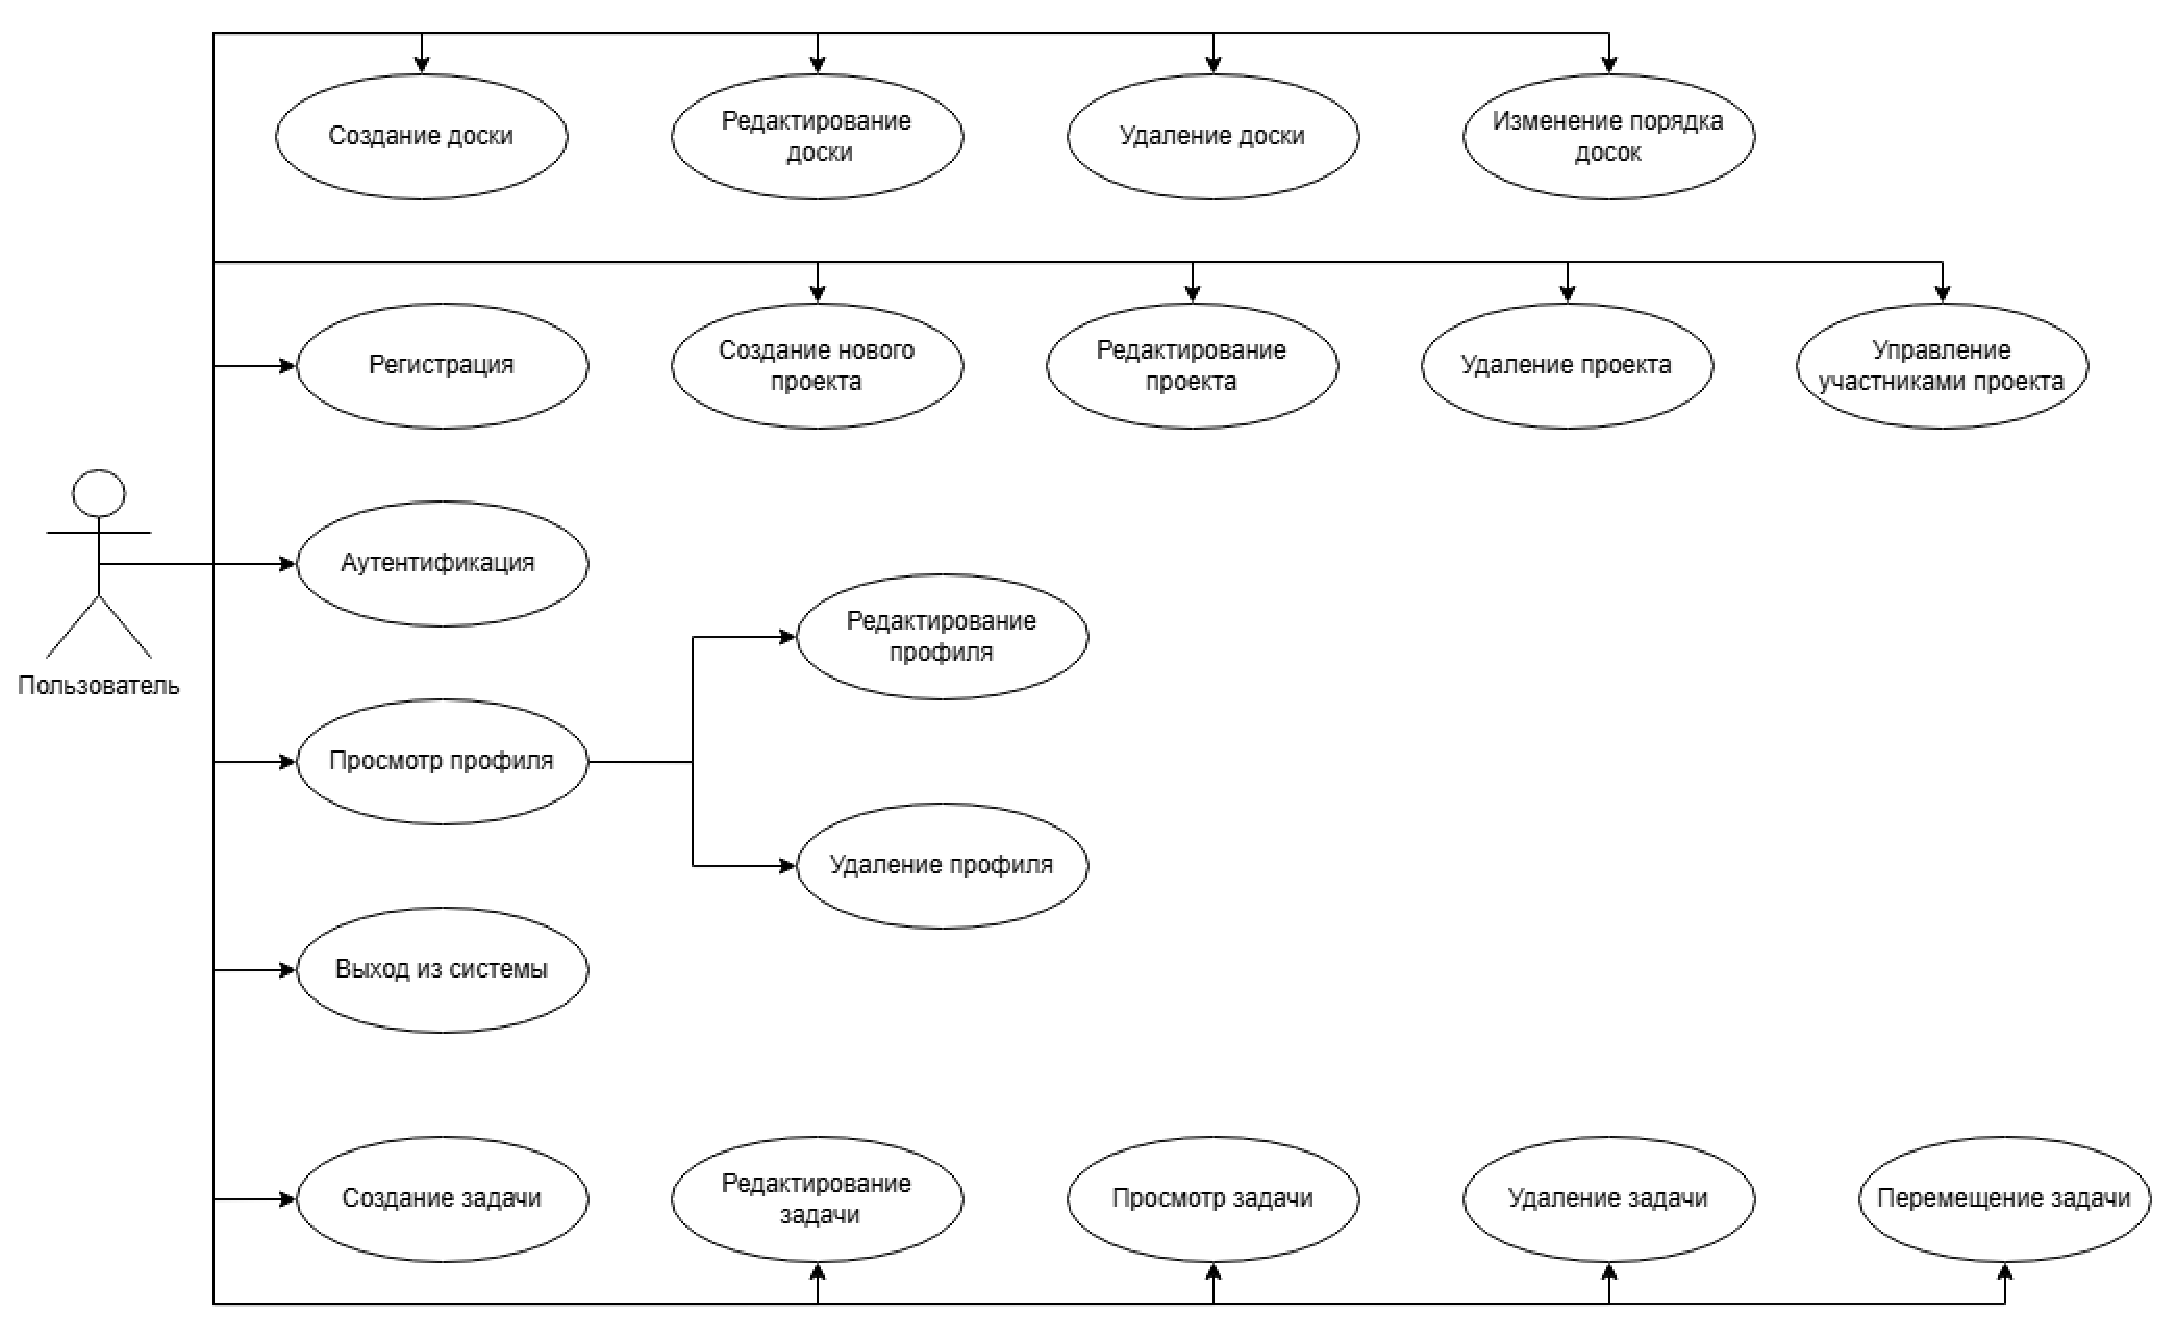
\includegraphics[width=1\linewidth]{use_case_diagram}
	\caption{Диаграмма прецедентов}
	\label{use_case_diagram:image}
\end{figure}


\subsubsection{Сценарий прецедента «Регистрация»}
Основной успешный сценарий:
\begin{itemize}
	\item Пользователь переходит на страницу аутентификации web-приложения.
	\item Пользователь нажимает на ссылку/кнопку «Создать».
	\item Пользователь вводит свое имя в поле «Имя».
	\item Пользователь вводит свою фамилию в поле «Фамилия».
	\item Пользователь вводит свой адрес электронной почты в поле «Адрес электронной почты».
	\item Пользователь вводит свой пароль в поле «Пароль», соблюдая указанные критерии.
	\item Пользователь подтверждает свой пароль в поле «Подтвердите пароль».
	\item Пользователь нажимает кнопку «Создать аккаунт».
	\item Система проверяет корректность введенных данных и уникальность email.
	\item Система регистрирует нового пользователя.
	\item Система автоматически аутентифицирует пользователя, сохраняет токен и перенаправляет его на основной интерфейс приложения (доску Kanban).
\end{itemize}

\subsubsection{Сценарий прецедента «Аутентификация»}
Основной успешный сценарий:
\begin{itemize}
	\item Пользователь переходит на страницу аутентификации web-приложения.
	\item Пользователь вводит свой адрес электронной почты в поле «Адрес электронной почты».
	\item Пользователь вводит свой пароль в поле «Пароль».
	\item Пользователь нажимает кнопку «Войти».
	\item Система проверяет корректность введенных учетных данных.
	\item Система аутентифицирует пользователя, сохраняет токен и перенаправляет его на основной интерфейс приложения (доску Kanban).
\end{itemize}

\subsubsection{Сценарий прецедента «Выход из системы»}
Основной успешный сценарий:
\begin{itemize}
	\item Аутентифицированный пользователь нажимает на иконку «Выйти» на панели настроек.
	\item Система отображает модальное окно с запросом подтверждения выхода.
	\item Пользователь нажимает кнопку «Выйти» в модальном окне.
	\item Система завершает сеанс пользователя (удаляет токен).
	\item Система перенаправляет пользователя на страницу аутентификации.
\end{itemize}

\subsubsection{Сценарий прецедента «Просмотр профиля»}
Основной успешный сценарий:
\begin{itemize}
	\item Аутентифицированный пользователь нажимает на иконку «Профиль пользователя» на панели настроек.
	\item Система отображает страницу профиля пользователя с его данными (ФИО, email, дата регистрации, аватар).
\end{itemize}

\subsubsection{Сценарий прецедента «Редактирование профиля»}
Основной успешный сценарий:
\begin{itemize}
	\item Пользователь находится на странице своего профиля.
	\item Пользователь нажимает кнопку «Редактировать профиль».
	\item Система отображает модальное окно редактирования профиля с текущими данными.
	\item Пользователь изменяет необходимые поля (имя, фамилия, отчество, URL аватара).
	\item Пользователь нажимает кнопку «Сохранить изменения».
	\item Система проверяет корректность введенных данных.
	\item Система обновляет данные профиля пользователя в базе данных.
	\item Система обновляет данные профиля в интерфейсе и закрывает модальное окно.
\end{itemize}

\subsubsection{Сценарий прецедента «Удаление профиля»}
Основной успешный сценарий:
\begin{itemize}
	\item Пользователь находится на странице своего профиля.
	\item Пользователь нажимает кнопку «Удалить профиль».
	\item Система отображает модальное окно с запросом подтверждения удаления профиля.
	\item Пользователь нажимает кнопку «Да, удалить мой профиль».
	\item Система удаляет профиль пользователя из базы данных.
	\item Система завершает сеанс пользователя и перенаправляет на страницу аутентификации.
\end{itemize}

\subsection*{Управление Проектами}

\subsubsection{Сценарий прецедента «Создание нового проекта»}
Основной успешный сценарий:
\begin{itemize}
	\item Аутентифицированный пользователь нажимает на иконку «Добавить новый проект» на панели настроек.
	\item Система отображает модальное окно для добавления проекта.
	\item Пользователь вводит название проекта в поле «Название проекта».
	\item Пользователь опционально вводит описание проекта в поле «Описание».
	\item Пользователь нажимает кнопку «Создать проект».
	\item Система создает новый проект в базе данных, назначая текущего пользователя владельцем.
	\item Система добавляет владельца в участники проекта.
	\item Система обновляет список проектов в интерфейсе, новый проект становится текущим (если это первый проект или по логике приложения).
	\item Модальное окно закрывается.
\end{itemize}

\subsubsection{Сценарий прецедента «Редактирование проекта»}
Условия: Пользователь является владельцем проекта или администратором.
Основной успешный сценарий:
\begin{itemize}
	\item Пользователь (владелец/админ) нажимает на иконку «Редактировать текущий проект» на панели настроек (кнопка активна, если проект выбран).
	\item Система отображает модальное окно редактирования текущего проекта с его данными.
	\item Пользователь изменяет название и/или описание проекта.
	\item Пользователь нажимает кнопку «Сохранить изменения».
	\item Система обновляет данные проекта в базе данных.
	\item Система обновляет название/описание проекта в интерфейсе. Модальное окно может закрыться или показать сообщение об успехе.
\end{itemize}

\subsubsection{Сценарий прецедента «Удаление проекта»}
Условия: Пользователь является владельцем проекта или администратором.
Основной успешный сценарий:
\begin{itemize}
	\item Пользователь (владелец/админ) открывает модальное окно редактирования проекта.
	\item Пользователь нажимает кнопку «Удалить проект».
	\item Система отображает модальное окно подтверждения удаления проекта.
	\item Пользователь нажимает кнопку «Да, удалить проект».
	\item Система удаляет проект, все связанные с ним доски и задачи из базы данных.
	\item Система обновляет список проектов в интерфейсе. Если удален текущий проект, выбирается другой или отображается состояние "нет проектов".
	\item Модальные окна закрываются.
\end{itemize}

\subsubsection{Сценарий прецедента «Управление участниками проекта»}
Условия: Пользователь является владельцем проекта или администратором.
Основной успешный сценарий (Просмотр):
\begin{itemize}
	\item Пользователь (владелец/админ) нажимает на иконку «Управление участниками проекта» на панели настроек (кнопка активна, если проект выбран).
	\item Система отображает модальное окно со списком текущих участников проекта.
\end{itemize}
Основной успешный сценарий (Добавление участника):
\begin{itemize}
	\item В модальном окне управления участниками пользователь вводит email существующего пользователя системы в поле «Введите email пользователя для добавления».
	\item Пользователь нажимает кнопку «Добавить».
	\item Система проверяет, существует ли пользователь с таким email и не является ли он уже участником.
	\item Система добавляет пользователя в участники проекта.
	\item Список участников в модальном окне обновляется.
\end{itemize}
Основной успешный сценарий (Удаление участника):
\begin{itemize}
	\item В модальном окне управления участниками пользователь нажимает иконку удаления напротив участника (не владельца).
	\item Система удаляет пользователя из участников проекта.
	\item Список участников в модальном окне обновляется.
\end{itemize}

\subsubsection{Сценарий прецедента «Создание доски»}
Условия: Пользователь является владельцем текущего проекта или администратором. Проект выбран.
Основной успешный сценарий:
\begin{itemize}
	\item Пользователь (владелец/админ) нажимает на иконку «Добавить новую доску» на панели настроек.
	\item Система отображает модальное окно для добавления доски.
	\item Пользователь вводит название доски в поле «Заголовок доски».
	\item Пользователь опционально вводит описание доски.
	\item Пользователь нажимает кнопку «Добавить доску».
	\item Система создает новую доску в текущем проекте.
	\item Система обновляет интерфейс, отображая новую доску в конце списка досок текущего проекта.
	\item Модальное окно закрывается.
\end{itemize}

\subsubsection{Сценарий прецедента «Редактирование доски»}
Условия: Пользователь является владельцем проекта, к которому принадлежит доска, или администратором.
Основной успешный сценарий:
\begin{itemize}
	\item Пользователь нажимает на иконку редактирования на заголовке доски.
	\item Система отображает модальное окно редактирования доски с ее текущими данными.
	\item Пользователь изменяет название и/или описание доски.
	\item Пользователь нажимает кнопку «Сохранить».
	\item Система обновляет данные доски в базе данных.
	\item Система обновляет отображение доски в интерфейсе. Модальное окно закрывается.
\end{itemize}

\subsubsection{Сценарий прецедента «Удаление доски»}
Условия: Пользователь является владельцем проекта, к которому принадлежит доска, или администратором.
Основной успешный сценарий:
\begin{itemize}
	\item Пользователь открывает модальное окно редактирования доски.
	\item Пользователь нажимает кнопку «Удалить доску».
	\item Система (опционально) запрашивает подтверждение.
	\item Система удаляет доску и все связанные с ней задачи.
	\item Система обновляет интерфейс, убирая доску. Модальное окно закрывается.
\end{itemize}

\subsubsection{Сценарий прецедента «Изменение порядка досок»}
Основной успешный сценарий:
\begin{itemize}
	\item Аутентифицированный пользователь наводит курсор на заголовок доски.
	\item Пользователь зажимает левую кнопку мыши на заголовке доски и перетаскивает доску на новую позицию среди других досок текущего проекта.
	\item Пользователь отпускает кнопку мыши.
	\item Система визуально обновляет порядок досок на экране.
	\item Система сохраняет новый порядок отображения досок для текущего проекта в базе данных.
\end{itemize}

\subsubsection{Сценарий прецедента «Создание  задачи»}
Условия: Пользователь аутентифицирован, проект выбран, и пользователь является участником проекта (или владельцем/администратором).
Основной успешный сценарий:
\begin{itemize}
	\item Пользователь нажимает на иконку «Добавить новую задачу» на панели настроек.
	\item Система отображает модальное окно для добавления задачи.
	\item Пользователь выбирает доску из выпадающего списка досок текущего проекта.
	\item Пользователь вводит заголовок задачи.
	\item Пользователь опционально вводит описание задачи.
	\item Пользователь выбирает срок выполнения, приоритет и тип задачи.
	\item Пользователь нажимает кнопку «Добавить задачу».
	\item Система создает новую задачу и связывает ее с выбранной доской и текущим проектом. Текущий пользователь назначается автором.
	\item Система обновляет интерфейс, отображая новую задачу на соответствующей доске.
	\item Модальное окно закрывается.
\end{itemize}

\subsubsection{Сценарий прецедента «Просмотр задачи»}
Основной успешный сценарий:
\begin{itemize}
	\item Аутентифицированный пользователь нажимает на карточку задачи на одной из досок.
	\item Система переключает вид основной области контента на страницу просмотра деталей задачи.
	\item На странице отображается полная информация о задаче: заголовок, описание, проект, доска, срок выполнения, приоритет, тип, автор, разработчик (если назначен), QA (если назначен).
\end{itemize}

\subsubsection{Сценарий прецедента «Редактирование задачи»}
Условия: Пользователь является автором задачи или администратором.
Основной успешный сценарий:
\begin{itemize}
	\item Пользователь находится на странице просмотра деталей задачи.
	\item Пользователь нажимает кнопку «Редактировать задачу».
	\item Система отображает модальное окно редактирования задачи с ее текущими данными (заголовок, описание, доска, приоритет; срок выполнения и тип НЕ редактируются в этой модали).
	\item Пользователь изменяет необходимые поля.
	\item Пользователь нажимает кнопку «Сохранить изменения».
	\item Система обновляет данные задачи в базе данных.
	\item Система обновляет отображение деталей задачи на странице и на карточке (если она видна). Модальное окно закрывается.
\end{itemize}

\subsubsection{Сценарий прецедента «Удаление задачи»}
Условия: Пользователь является автором задачи или администратором.
Основной успешный сценарий:
\begin{itemize}
	\item Пользователь находится на странице просмотра деталей задачи.
	\item Пользователь нажимает кнопку «Удалить задачу».
	\item Система отображает модальное окно подтверждения удаления.
	\item Пользователь нажимает кнопку «Да, удалить».
	\item Система удаляет задачу из базы данных.
	\item Система перенаправляет пользователя на доску Kanban и обновляет интерфейс.
\end{itemize}

\subsubsection{Сценарий прецедента «Перемещение задачи»}
Основной успешный сценарий:
\begin{itemize}
	\item Аутентифицированный пользователь наводит курсор на карточку задачи.
	\item Пользователь зажимает левую кнопку мыши на карточке задачи и перетаскивает ее на другую доску в рамках текущего проекта.
	\item Пользователь отпускает кнопку мыши над целевой доской.
	\item Система визуально перемещает карточку задачи на новую доску и обновляет ее позицию в списке задач новой доски.
	\item Система обновляет board\_id и display\_order задачи в базе данных.
\end{itemize}

\subsection{Требования пользователя к интерфейсу web-интерфейса}
Интерфейс должен быть интуитивно понятным, чтобы пользователи могли легко взаимодействовать с системой.
На рисунке ~\ref{page_example:image} представлен макет страницы.

\begin{figure}[H]
	\centering
	\includegraphics[width=0.9\linewidth]{page_example}
	\caption{Макет страницы}
	\label{page_example:image}
\end{figure}

\subsection{Нефункциональные требования}

\subsubsection{Требования к программному обеспечению}

Для разработки и полноценной работы системы управления проектами необходимы следующие программные компоненты:

\begin{enumerate}
	\item Среда выполнения JavaScript - Node.js.
	\item Инструмент для сборки и разработки на основе Node.js - Vite.
	\item Библиотека React для построения пользовательских интерфейсов.
	\item Библиотека Zustand для управления состоянием приложения.
	\item Библиотека react-beautiful-dnd для реализации функциональности перетаскивания.
	\item CSS-фреймворк Tailwind CSS для стилизации интерфейса.
	\item Вспомогательные JavaScript-библиотеки:
	\begin{itemize}
		\item для генерации уникальных идентификаторов - uuid.
		\item для проверки типов свойств React-компонентов - prop-types.
	\end{itemize}
\end{enumerate}

\subsection{Ограничения}

\begin{enumerate}
	\item Для доступа ко всем функциям системы, включая совместную работу и синхронизацию данных в реальном времени, необходимо постоянное и стабильное подключение к сети Интернет.
	\item Система ориентирована на управление проектами с использованием Kanban-методологии и может не покрывать все потребности проектов, требующих других подходов или расширенного инструментария (например, диаграмм Ганта или сложного финансового учета).
	\item Точность и эффективность специфических аналитических функций напрямую зависят от полноты, актуальности и качества данных, вводимых пользователями в систему.
	\item Производительность системы при работе с очень большим количеством одновременных пользователей или значительными объемами данных (множество проектов, досок, задач) будет зависеть от характеристик и масштабируемости серверной инфраструктуры.
\end{enumerate}

\subsubsection{Требования к аппаратному обеспечению}
Для работы приложения требуется дисковое пространство не менее 5 Гб, минимум 16 Гб оперативной памяти и подключение к Интернету. Рекомендуется использовать процессор c 6 или более ядрами и частотой 2 ГГц или выше.

\subsection{Требования к оформлению документации}

Разработка программной документации и программного изделия должна производиться согласно ГОСТ 19.102-77 и ГОСТ 34.601-90. Единая система программной документации.

\section{Технический проект}
\subsection{Общая характеристика организации решения задачи}

Задача заключается в разработке и программной реализации веб-приложения для управления проектами, основанного на использовании Kanban-доски и принципов Agile-методологий. Приложение предназначено для командной работы и поможет руководителям проектов, а также членам команд эффективно планировать спринты и текущую деятельность, визуализировать рабочие процессы, отслеживать выполнение задач и улучшать взаимодействие, что способствует повышению общей продуктивности и успешности проектов.

Приложение будет представлять собой многопользовательский веб-сервис, доступный через сеть Интернет. Основными элементами интерфейса будут являться интерактивная Kanban-доска для визуального управления задачами, страницы для настройки проектов и досок, а также инструменты для поддержки Agile-практик, такие как управление бэклогом и отслеживание прогресса по итерациям.

\subsection{Обоснование выбора технологии проектирования}

Для создания приложения выбраны технологии, которые обеспечивают высокую производительность и удобство для пользователей.

\subsubsection{Язык программирования JavaScript}
JavaScript — это высокоуровневый, мультипарадигменный язык программирования, являющийся ключевой технологией для создания интерактивных веб-сайтов и приложений. Он выполняется непосредственно в браузере пользователя, обеспечивая динамическое обновление контента и взаимодействие без перезагрузки страницы, а также может использоваться на серверной стороне благодаря среде Node.js \cite{javascript1}.

\subsubsection{Среда выполнения Node.js}
Node.js — это кроссплатформенная среда выполнения JavaScript, построенная на движке V8 от Google Chrome. Она позволяет исполнять JavaScript-код на стороне сервера, что открывает возможности для создания быстрых и масштабируемых сетевых приложений \cite{nodejs1}.

\subsubsection{Библиотека React}
React — это популярная JavaScript-библиотека для создания пользовательских интерфейсов, разработанная и поддерживаемая Facebook (ныне Meta). В основе React лежит концепция компонентного подхода, позволяющая разбивать сложный интерфейс на независимые, переиспользуемые части — компоненты, каждый из которых управляет собственным состоянием \cite{react1}.

\subsubsection{PostgreSQL}

PostgreSQL — это объектно-реляционная система управления базами данных, известная своей надежностью, гибкостью и расширяемостью. Она поддерживает широкий спектр функциональности, включая сложные запросы, транзакции, уровни изоляции и возможность создания пользовательских типов данных \cite{postgres1}.

\subsection{Диаграмма компонентов}

 На рисунке \ref{components_diagram.eps:image} изображена диаграмма компонентов системы.
 
 \begin{figure}[ht]
 	\center{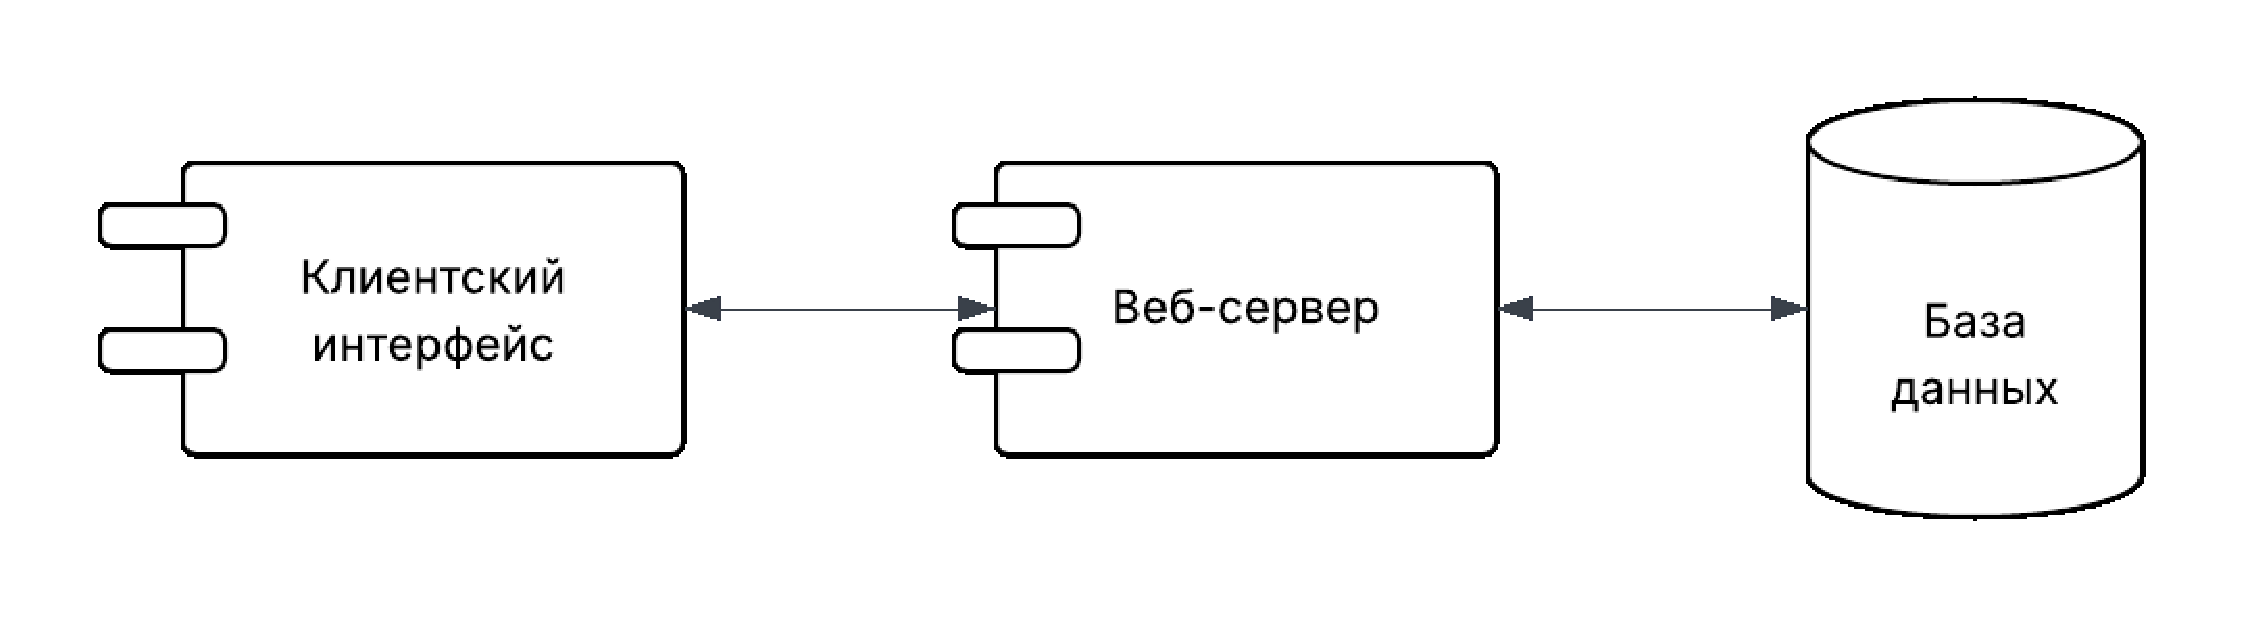
\includegraphics[width=1\linewidth]{components_diagram}}
 	\caption{Диаграмма компонентов}
 	\label{components_diagram.eps:image}
 \end{figure}
 
 На представленной диаграмме показана архитектура веб-приложения для управления проектами, основанного на Kanban-доске и Agile-методиках. Схема включает три основных компонента: «Клиентский интерфейс», «Веб-сервер» и «База данных». Эти компоненты соединены стрелками, которые указывают направление потоков данных и взаимодействия между ними. Каждая часть системы выполняет свои специфические функции, обеспечивая совместную и эффективную работу всего приложения.
 
 «Клиентский интерфейс» — это веб-приложение, которое запускается в браузере пользователя и служит основной точкой взаимодействия с системой. Через него пользователи могут регистрироваться и аутентифицироваться, создавать новые проекты, настраивать Kanban-доски, добавлять, редактировать и перемещать задачи между колонками. На страницах интерфейса в реальном времени отображается актуальное состояние проектов, Kanban-доски, списки задач, бэклоги и другая информация, необходимая для организации работы по Agile-принципам.
 
 «Веб-сервер» функционирует как центральный узел архитектуры, обрабатывающий всю бизнес-логику системы. Он получает HTTP-запросы от «Клиентского интерфейса», выполняет соответствующие операции, взаимодействует с «Базой данных» для сохранения или извлечения необходимой информации, и отправляет ответы «Клиентскому интерфейсу» для обновления отображаемых данных или подтверждения выполненных действий.
 
 «База данных» отвечает за надежное и долговременное хранение всей информации, используемой в системе управления проектами. В ней содержатся структурированные данные о зарегистрированных пользователях, созданных проектах, деталях задач, конфигурациях Kanban-досок и другие сведения, необходимые для функционирования Agile-процессов. «Веб-сервер» постоянно обращается к «Базе данных» для выполнения операций чтения и записи данных при каждом значимом взаимодействии пользователя с системой.
 
\subsection{Структура программы}
Система управления проектами представляет собой веб-приложение, чья структура организована в виде набора модулей, каждый из которых выполняет определённые функции.
\subsubsection{Клиентская часть}
Клиентская часть приложения разработана с использованием библиотеки React и отвечает за пользовательский интерфейс и взаимодействие с пользователем. Она включает в себя набор компонентов, каждый из которых выполняет определенную функцию, начиная от отображения основных элементов управления и заканчивая сложными модальными окнами для управления данными:
\begin{enumerate}
	\item Модуль App.jsx. Главный компонент React-приложения. Управляет состоянием аутентификации пользователя, маршрутизацией между основными представлениями, отображением глобальных модальных окон. Инициализирует загрузку основных данных при входе пользователя и при их обновлении.
	\item Модуль Layout.jsx. Компонент, определяющий основной макет интерфейса для аутентифицированных пользователей. Включает боковую панель настроек, верхнюю панель со списком проектов и поиском, а также основную область контента, где динамически отображаются либо доски Kanban с задачами, либо страница детального просмотра задачи. Реализует логику перетаскивания для досок и задач.
	\item Модуль AuthPage.jsx. Компонент страницы аутентификации. Предоставляет пользователю интерфейс для регистрации новой учетной записи и входа в существующую. Включает валидацию вводимых данных и отображение требований к паролю.
	\item Модуль UserProfilePage.jsx. Компонент страницы профиля пользователя. Отображает информацию о текущем аутентифицированном пользователе и предоставляет функционал для редактирования и удаления профиля через соответствующие модальные окна.
	\item Модуль TaskViewPage.jsx. Компонент страницы детального просмотра задачи. Отображает всю информацию о выбранной задаче, включая ее заголовок, описание, проект, доску, срок выполнения, приоритет, тип, автора, а также назначенных разработчика и QA-специалиста. Предоставляет пользователю возможность назначить себя на роль разработчика или QA, если эти роли свободны. Также содержит кнопки для редактирования и удаления задачи.
	\item Модуль Board.jsx. Компонент, представляющий одну доску Kanban в рамках проекта. Отображает заголовок и описание доски. Содержит список задач, принадлежащих этой доске, и обеспечивает возможность перетаскивания задач. Предоставляет кнопку для редактирования/удаления доски.
	\item Модуль Task.jsx. Компонент, представляющий карточку отдельной задачи на доске. Отображает заголовок задачи, ее тип, приоритет, срок выполнения, а также краткую информацию об авторе, разработчике и QA-специалисте. Позволяет пользователю кликнуть по карточке для перехода на страницу детального просмотра задачи.
	\item Модуль SettingsPanel.jsx. Компонент боковой панели навигации и действий. Содержит кнопки для добавления новой задачи, перехода к профилю пользователя, добавления нового проекта, добавления новой доски, редактирования текущего проекта, управления участниками текущего проекта и выхода из системы. Видимость некоторых кнопок зависит от роли пользователя и выбранного проекта.
	\item Модуль ProjectListBar.jsx. Компонент, отображаемый в верхней части интерфейса. Содержит выпадающий список для выбора текущего проекта из числа тех, в которых пользователь состоит.
	\item Модуль Tooltip.jsx. Вспомогательный компонент для отображения всплывающих текстовых подсказок при наведении курсора на элементы интерфейса.
	\item Модуль Modal.jsx. Компонент модального окна для создания новой задачи. Позволяет выбрать доску, ввести заголовок, описание, срок выполнения, а также выбрать приоритет и тип задачи.
	\item Модуль ModalAddBoard.jsx. Компонент модального окна для добавления новой доски в выбранный проект. Позволяет ввести заголовок и описание доски.
	\item Модуль ModalAddProject.jsx. Компонент модального окна для создания нового проекта. Позволяет ввести название и описание проекта.
	\item Модуль ModalAlert.jsx. Общий компонент для отображения простых информационных сообщений или оповещений об ошибках с одной кнопкой «OK».
	\item Модуль ModalConfirm.jsx. Общий компонент для запроса подтверждения у пользователя перед выполнением деструктивных или важных действий. Предоставляет кнопки «Подтвердить» и «Отмена».
	\item Модуль ModalEditBoard.jsx. Компонент модального окна для редактирования существующей доски. Позволяет изменить заголовок и описание доски, а также удалить доску.
	\item Модуль ModalEditProfile.jsx. Компонент модального окна для редактирования персональной информации пользователя.
	\item Модуль ModalEditProject.jsx. Компонент модального окна для редактирования существующего проекта. Позволяет изменить название и описание проекта, а также удалить проект.
	\item Модуль ModalEditTask.jsx. Компонент модального окна для редактирования существующей задачи. Позволяет изменить заголовок, описание, доску и приоритет задачи.
	\item Модуль ModalManageProjectMembers.jsx. Компонент модального окна для управления участниками выбранного проекта. Позволяет просматривать список участников, добавлять новых участников по email и удалять существующих.
\end{enumerate}

\subsubsection{Серверная часть}
Серверная часть приложения, построенная на Node.js с использованием фреймворка Express.js, обеспечивает обработку всех API-запросов, управление бизнес-логикой, взаимодействие с базой данных и реализацию механизмов безопасности, таких как аутентификация и авторизация. Списко связанных модулей:
\begin{enumerate}
	\item Модуль server.js. Основной файл серверной части приложения, реализованный на Node.js с использованием фреймворка Express.js. Отвечает за обработку всех API-запросов от клиентской части. Реализует эндпоинты для:
	\begin{itemize}
		\item регистрации и аутентификации пользователей;
		\item управления профилями пользователей;
		\item получения списка всех пользователей системы;
		\item управления проектами;
		\item управления участниками проектов;
		\item управления досками;
		\item управления задачами.
	\end{itemize}

Взаимодействует с базой данных PostgreSQL для хранения и извлечения данных. Реализует логику авторизации, проверяя права пользователя (например, владелец проекта, администратор, участник проекта) перед выполнением защищенных операций.
\end{enumerate}

\subsubsection{Клиентские сервисы}
Клиентские сервисы представляют собой вспомогательные JavaScript-модули, которые инкапсулируют специфическую логику, используемую различными компонентами клиентской части. Они помогают упростить взаимодействие с API и управление состоянием аутентификации. Список связанных модулей:
\begin{enumerate}
	\item Модуль apiService.js. Модуль на стороне клиента, предоставляющий функцию authenticatedFetch для упрощения выполнения аутентифицированных HTTP-запросов к API серверной части. Автоматически добавляет JWT токен аутентификации в заголовки запросов. Содержит логику для обработки специфических ошибок от сервера и вызова глобального обработчика для принудительного выхода пользователя из системы при проблемах с сессией или токеном.
	\item Модуль tokenService.js. Модуль на стороне клиента, предоставляющий утилиты для работы с JWT токеном. Включает функцию isTokenActive для проверки наличия токена в localStorage и валидации его срока действия путем декодирования с использованием jwt-decode.
\end{enumerate}

\subsubsection{Управление состоянием и стилизация}
Для эффективного управления состоянием приложения на стороне клиента используется библиотека Zustand, обеспечивающая централизованное и реактивное хранилище данных. Визуальное оформление реализуется с помощью Tailwind CSS и кастомных CSS-правил для создания консистентного и адаптивного пользовательского интерфейса. Список связанных модулей:
\begin{enumerate}
	\item Модуль store.js. Файл, определяющий глобальное хранилище состояния приложения с использованием библиотеки Zustand. Содержит состояние для проектов, досок, задач, информации о текущем пользователе, списке всех пользователей, текущем выбранном проекте и задаче, виде отображения приложения, а также различные флаги для модальных окон и оповещений. Реализует действия для изменения этого состояния. Использует middleware persist для сохранения части состояния в localStorage браузера.
	\item Модуль index.css. Основной файл стилей приложения. Включает базовые стили и утилиты Tailwind CSS, а также кастомные CSS-правила для оформления полос прокрутки и других элементов интерфейса для обеспечения единого визуального стиля.
\end{enumerate}

\subsubsection{Точка входа и конфигурация БД}
Этот раздел описывает основные файлы, отвечающие за запуск клиентского приложения, а также скрипт для инициализации и настройки структуры базы данных PostgreSQL, включая создание таблиц и заполнение начальными данными. Список связанных элементов:
\begin{enumerate}
	\item Модуль main.jsx. Точка входа клиентского React-приложения. Инициализирует корневой компонент App и рендерит его в DOM-элемент с id root. Подключает основные стили из index.css.
	\item db\_schema.sql. SQL-скрипт, предназначенный для инициализации структуры базы данных PostgreSQL. Содержит команды создания для всех необходимых сущностей, определяет первичные и внешние ключи, ограничения, значения по умолчанию и триггеры для автоматического обновления временных меток. Также включает секцию для заполнения базы данных начальными тестовыми данными для демонстрации и тестирования функционала.
\end{enumerate}

\subsection{Структура базы данных}
Сущности и отношения между ними отображены на ER-диаграмме.
\newpage
 \begin{figure}[ht]
	\center{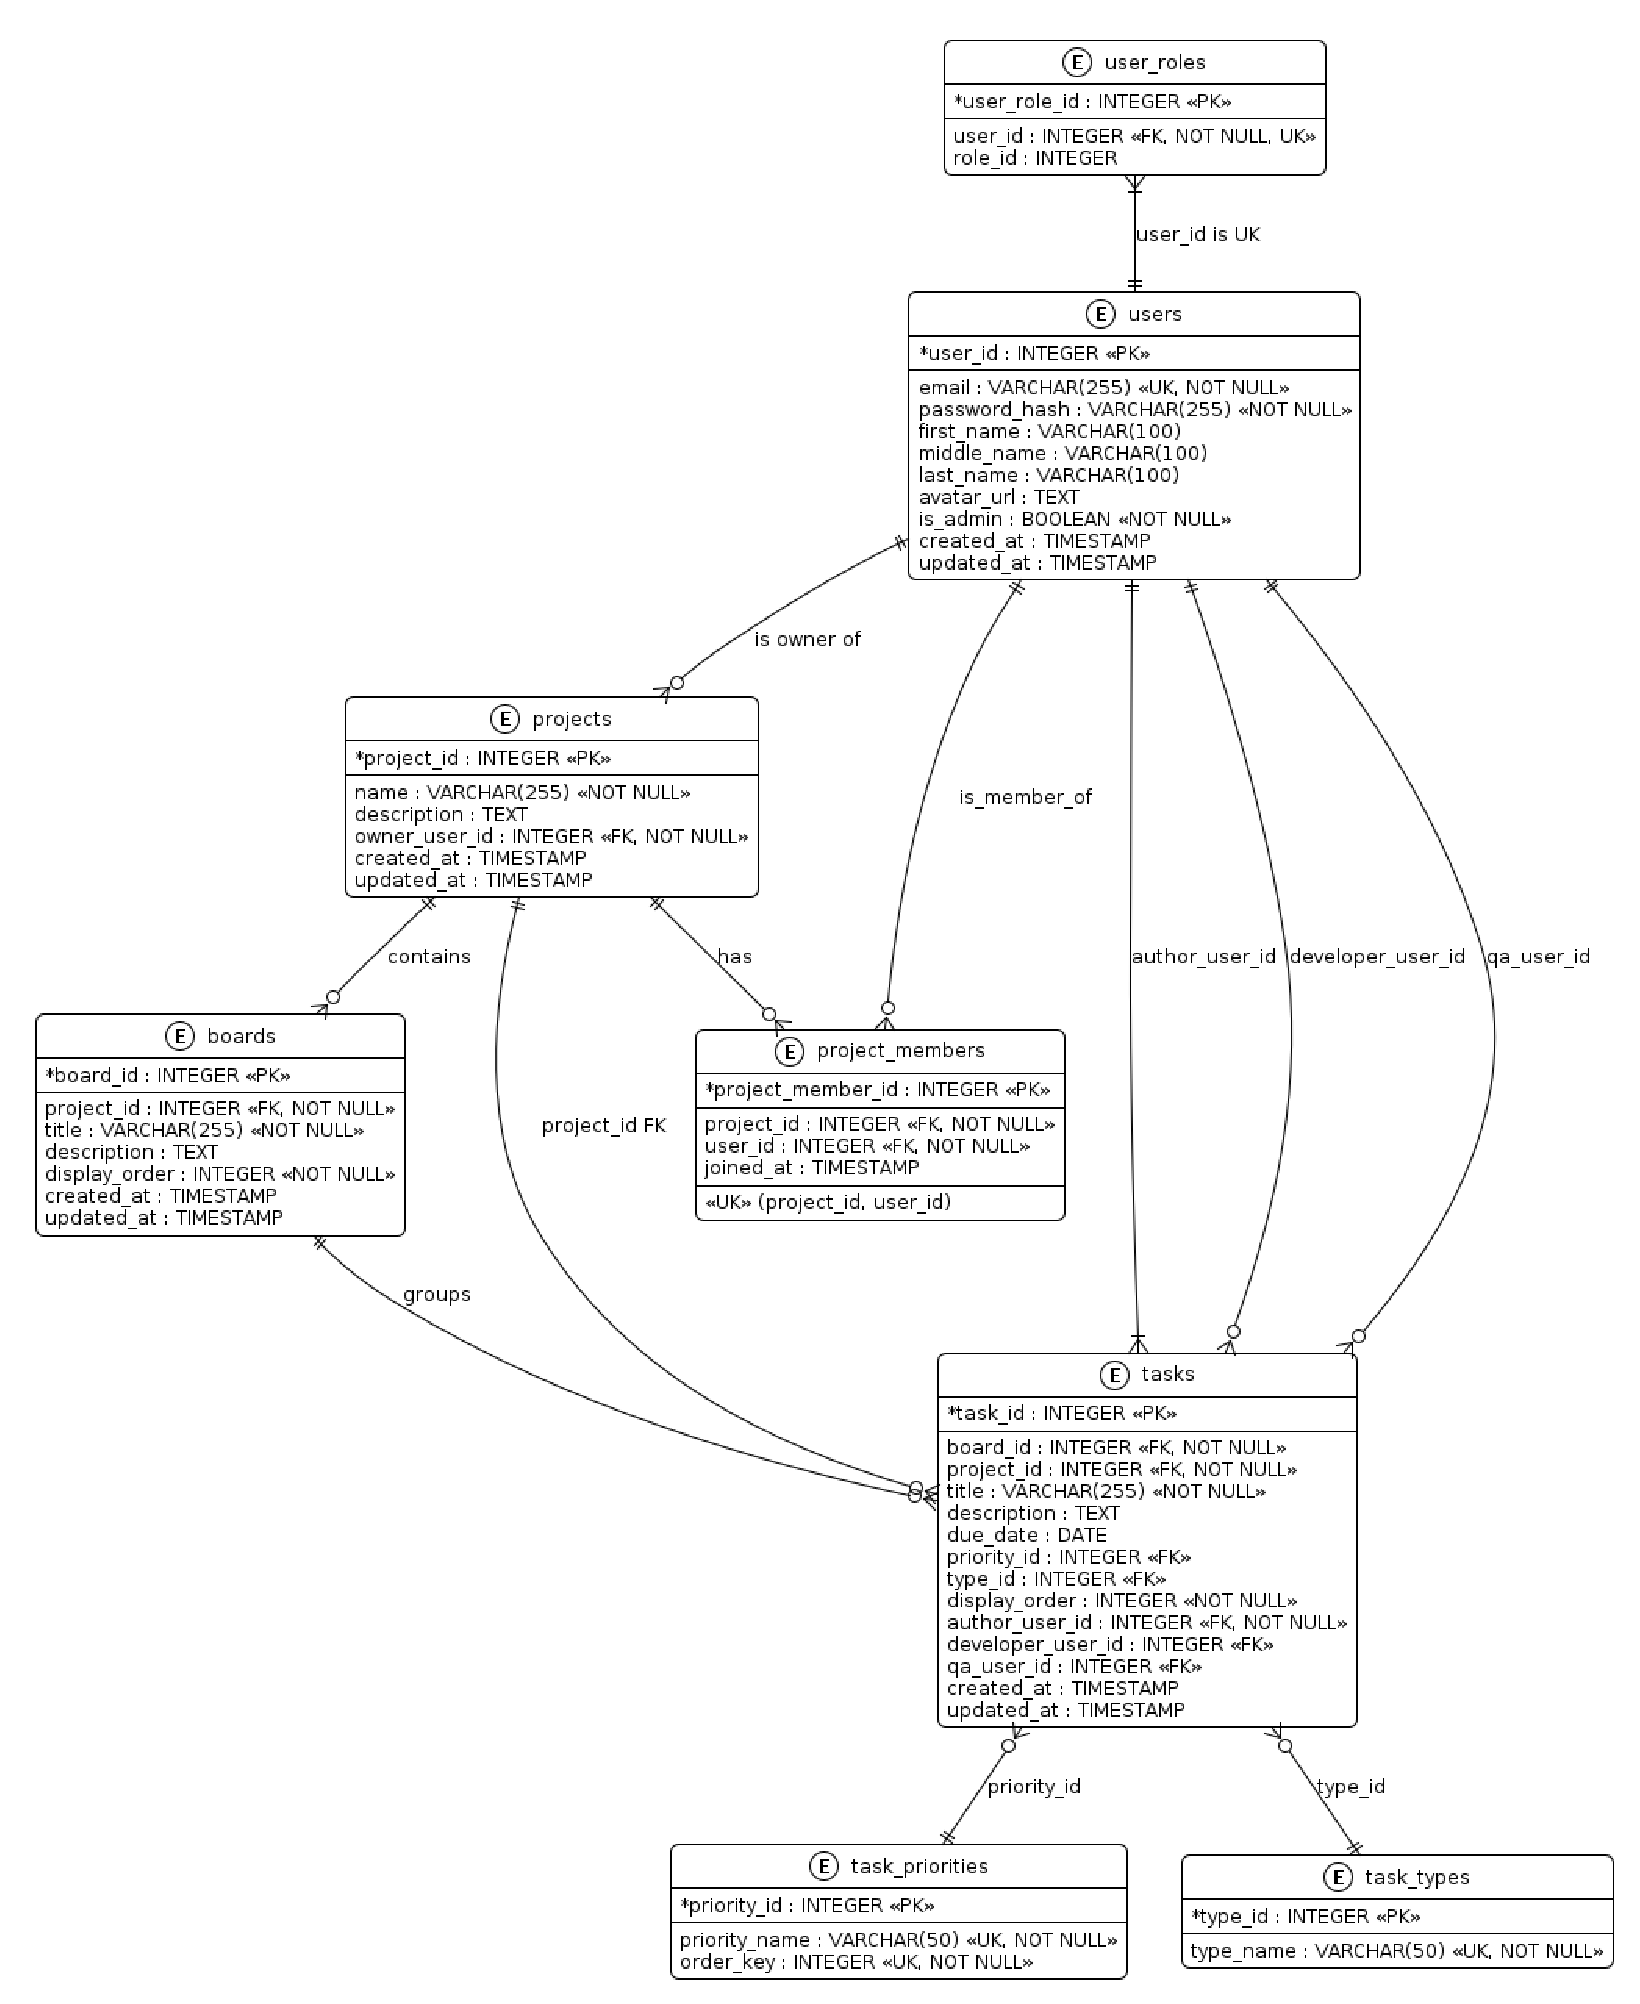
\includegraphics[width=1\linewidth]{er_diagram}}
	\caption{ER-диаграмма}
	\label{er_diagram:image}
\end{figure}
\newpage
\begin{xltabular}{\textwidth}{|p{2.5cm}|p{4cm}|p{1.7cm}|X|}
	\caption{Атрибуты сущности «Users»\label{users:table}}\\ \hline
	\centrow Поле & \centrow Тип & \centrow Обяза\-тельное & \centrow Описание \\ \hline
	\thead{1} & \thead{2} & \centrow 3 & \centrow 4 \\ \hline
	\endfirsthead
	\caption*{Продолжение таблицы \ref{users:table}} \\ \hline
	\thead{1} & \thead{2} & \centrow 3 & \centrow 4 \\ \hline
	\finishhead
	user\_id & SERIAL, PK & \centrow да & Первичный ключ, уникальный идентификатор пользователя. \\ \hline
	email & VARCHAR(255), UNIQUE, NOT NULL & \centrow да & Адрес электронной почты пользователя, уникальный. \\ \hline
	password\_ hash & VARCHAR(255), NOT NULL & \centrow да & Хеш пароля пользователя. \\ \hline
	first\_name & VARCHAR(100) & \centrow нет & Имя пользователя. \\ \hline
	middle\_ name & VARCHAR(100) & \centrow нет & Отчество пользователя. \\ \hline
	last\_name & VARCHAR(100) & \centrow нет & Фамилия пользователя. \\ \hline
	avatar\_url & TEXT & \centrow нет & URL-адрес аватара пользователя. \\ \hline
	is\_admin & BOOLEAN, DEFAULT FALSE, NOT NULL & \centrow да & Флаг, указывающий, является ли пользователь администратором. \\ \hline
	created\_at & TIMESTAMP WITH TIME ZONE, DEFAULT CURRENT\_ TIMESTAMP & \centrow да & Дата и время создания записи. \\ \hline
	updated\_at & TIMESTAMP WITH TIME ZONE, DEFAULT CURRENT\_ TIMESTAMP & \centrow да & Дата и время последнего обновления записи. \\ \hline
\end{xltabular}

\begin{xltabular}{\textwidth}{|p{2.5cm}|p{4cm}|p{1.7cm}|X|}
	\caption{Атрибуты сущности «Projects»\label{projects:table}}\\ \hline
	\centrow Поле & \centrow Тип & \centrow Обяза\-тельное & \centrow Описание \\ \hline
	\thead{1} & \thead{2} & \centrow 3 & \centrow 4 \\ \hline
	\endfirsthead
	\caption*{Продолжение таблицы \ref{projects:table}} \\ \hline
	\thead{1} & \thead{2} & \centrow 3 & \centrow 4 \\ \hline
	\finishhead
	project\_id & SERIAL, PK & \centrow да & Первичный ключ, уникальный идентификатор проекта. \\ \hline
	name & VARCHAR(255), NOT NULL & \centrow да & Название проекта. \\ \hline
	description & TEXT & \centrow нет & Описание проекта. \\ \hline
	owner\_ user\_id & INTEGER, FK, NOT NULL & \centrow да & Внешний ключ, ссылается на users(user\_id). Идентификатор пользователя-владельца проекта. \\ \hline
	created\_at & TIMESTAMP WITH TIME ZONE, DEFAULT CURRENT\_ TIMESTAMP & \centrow да & Дата и время создания записи. \\ \hline
	updated\_at & TIMESTAMP WITH TIME ZONE, DEFAULT CURRENT\_ TIMESTAMP & \centrow да & Дата и время последнего обновления записи. \\ \hline
\end{xltabular}

\begin{xltabular}{\textwidth}{|p{2.5cm}|p{4cm}|p{1.7cm}|X|}
	\caption{Атрибуты сущности «Project Members»\label{projectmembers:table}}\\ \hline
	\centrow Поле & \centrow Тип & \centrow Обяза\-тельное & \centrow Описание \\ \hline
	\thead{1} & \thead{2} & \centrow 3 & \centrow 4 \\ \hline
	\endfirsthead
	\caption*{Продолжение таблицы \ref{projectmembers:table}} \\ \hline
	\thead{1} & \thead{2} & \centrow 3 & \centrow 4 \\ \hline
	\finishhead
	project\_ member\_id & SERIAL, PK & \centrow да & Первичный ключ, уникальный идентификатор записи об участии. \\ \hline
	project\_id & INTEGER, FK, NOT NULL & \centrow да & Внешний ключ, ссылается на projects(project\_id). Идентификатор проекта. \\ \hline
	user\_id & INTEGER, FK, NOT NULL & \centrow да & Внешний ключ, ссылается на users(user\_id). Идентификатор пользователя-участника. \\ \hline
	joined\_at & TIMESTAMP WITH TIME ZONE, DEFAULT CURRENT\_ TIMESTAMP & \centrow да & Дата и время присоединения пользователя к проекту. \\ 
	\hline
\end{xltabular}

\begin{xltabular}{\textwidth}{|p{2.5cm}|p{4cm}|p{1.7cm}|X|}
	\caption{Атрибуты сущности «Boards»\label{boards:table}}\\ \hline
	\centrow Поле & \centrow Тип & \centrow Обяза\-тельное & \centrow Описание \\ \hline
	\thead{1} & \thead{2} & \centrow 3 & \centrow 4 \\ \hline
	\endfirsthead
	\caption*{Продолжение таблицы \ref{boards:table}} \\ \hline
	\thead{1} & \thead{2} & \centrow 3 & \centrow 4 \\ \hline
	\finishhead
	board\_id & SERIAL, PK & \centrow да & Первичный ключ, уникальный идентификатор доски. \\ \hline
	project\_id & INTEGER, FK, NOT NULL & \centrow да & Внешний ключ, ссылается на projects(project\_id). Идентификатор проекта, к которому принадлежит доска. \\ \hline
	title & VARCHAR(255), NOT NULL & \centrow да & Название доски. \\ \hline
	description & TEXT & \centrow нет & Описание доски. \\ \hline
	display\_order & INTEGER, NOT NULL, DEFAULT 0 & \centrow да & Порядок отображения доски в проекте. \\ \hline
	created\_at & TIMESTAMP WITH TIME ZONE, DEFAULT CURRENT\_ TIMESTAMP & \centrow да & Дата и время создания записи. \\ \hline
	updated\_at & TIMESTAMP WITH TIME ZONE, DEFAULT CURRENT\_ TIMESTAMP & \centrow да & Дата и время последнего обновления записи. \\ \hline
\end{xltabular}

\begin{xltabular}{\textwidth}{|p{2.5cm}|p{4cm}|p{1.7cm}|X|}
	\caption{Атрибуты сущности «Task Priorities»\label{taskpriorities:table}}\\ \hline
	\centrow Поле & \centrow Тип & \centrow Обяза\-тельное & \centrow Описание \\ \hline
	\thead{1} & \thead{2} & \centrow 3 & \centrow 4 \\ \hline
	\endfirsthead
	\caption*{Продолжение таблицы \ref{taskpriorities:table}} \\ \hline
	\thead{1} & \thead{2} & \centrow 3 & \centrow 4 \\ \hline
	\finishhead
	priority\_id & SERIAL, PK & \centrow да & Первичный ключ, уникальный идентификатор приоритета. \\ \hline
	priority\_ name & VARCHAR(50), UNIQUE, NOT NULL & \centrow да & Название приоритета (например, 'Low', 'Medium'). \\ \hline
	order\_key & INTEGER, UNIQUE, NOT NULL & \centrow да & Ключ для сортировки приоритетов. \\ \hline
\end{xltabular}

\begin{xltabular}{\textwidth}{|p{2.5cm}|p{4cm}|p{1.7cm}|X|}
	\caption{Атрибуты сущности «Task Types»\label{tasktypes:table}}\\ \hline
	\centrow Поле & \centrow Тип & \centrow Обяза\-тельное & \centrow Описание \\ \hline
	\thead{1} & \thead{2} & \centrow 3 & \centrow 4 \\ \hline
	\endfirsthead
	\caption*{Продолжение таблицы \ref{tasktypes:table}} \\ \hline
	\thead{1} & \thead{2} & \centrow 3 & \centrow 4 \\ \hline
	\finishhead
	type\_id & SERIAL, PK & \centrow да & Первичный ключ, уникальный идентификатор типа задачи. \\ \hline
	type\_name & VARCHAR(50), UNIQUE, NOT NULL & \centrow да & Название типа задачи (например, 'FRONTEND', 'BUGFIX'). \\ \hline
\end{xltabular}

\begin{xltabular}{\textwidth}{|p{2.5cm}|p{4cm}|p{1.7cm}|X|}
	\caption{Атрибуты сущности «Tasks»\label{tasks:table}}\\ \hline
	\centrow Поле & \centrow Тип & \centrow Обяза\-тельное & \centrow Описание \\ \hline
	\thead{1} & \thead{2} & \centrow 3 & \centrow 4 \\ \hline
	\endfirsthead
	\caption*{Продолжение таблицы \ref{tasks:table}} \\ \hline
	\thead{1} & \thead{2} & \centrow 3 & \centrow 4 \\ \hline
	\finishhead
	task\_id & SERIAL, PK & \centrow да & Первичный ключ, уникальный идентификатор задачи. \\ \hline
	board\_id & INTEGER, FK, NOT NULL & \centrow да & Внешний ключ, ссылается на boards(board\_id). Идентификатор доски, на которой находится задача. \\ \hline
	project\_id & INTEGER, FK, NOT NULL & \centrow да & Внешний ключ, ссылается на projects(project\_id). Идентификатор проекта, к которому принадлежит задача. \\ \hline
	title & VARCHAR(255), NOT NULL & \centrow да & Заголовок задачи. \\ \hline
	description & TEXT & \centrow нет & Описание задачи. \\ \hline
	due\_date & DATE & \centrow нет & Срок выполнения задачи. \\ \hline
	priority\_id & INTEGER, FK & \centrow нет & Внешний ключ, ссылается на task\_priorities(priority\_id). Идентификатор приоритета задачи. \\ \hline
	type\_id & INTEGER, FK & \centrow нет & Внешний ключ, ссылается на task\_types(type\_id). Идентификатор типа задачи. \\ \hline
	display\_ order & INTEGER, NOT NULL, DEFAULT 0 & \centrow да & Порядок отображения задачи на доске. \\ \hline
	author\_ user\_id & INTEGER, FK, NOT NULL & \centrow да & Внешний ключ, ссылается на users(user\_id). Идентификатор пользователя-автора задачи. \\ \hline
	developer\_ user\_id & INTEGER, FK & \centrow нет & Внешний ключ, ссылается на users(user\_id). Идентификатор пользователя-разработчика. \\ \hline
	qa\_user\_id & INTEGER, FK & \centrow нет & Внешний ключ, ссылается на users(user\_id). Идентификатор пользователя-тестировщика. \\ \hline
	created\_at & TIMESTAMP WITH TIME ZONE, DEFAULT CURRENT\_ TIMESTAMP & \centrow да & Дата и время создания записи. \\ \hline
	updated\_at & TIMESTAMP WITH TIME ZONE, DEFAULT CURRENT\_ TIMESTAMP & \centrow да & Дата и время последнего обновления записи. \\ \hline
\end{xltabular}
\ifПрактика{}\else{
   \section{Рабочий проект}
\subsection{Классы, используемые при разработке сайта}

Можно выделить следующий список классов и их методов, использованных при разработке web-приложения (таблица \ref{class:table}). Пример таблицы с уменьшенным межстрочным интервалом.

\renewcommand{\arraystretch}{0.8} % уменьшение расстояний до сетки таблицы
\begin{xltabular}{\textwidth}{|X|p{2.5cm}|>{\setlength{\baselineskip}{0.7\baselineskip}}p{4.85cm}|>{\setlength{\baselineskip}{0.7\baselineskip}}p{4.85cm}|}
\caption{Описание классов Bitrix, используемых в приложении\label{class:table}}\\
\hline \centrow \setlength{\baselineskip}{0.7\baselineskip} Название класса & \centrow \setlength{\baselineskip}{0.7\baselineskip} Модуль, к которому относится класс & \centrow Описание класса & \centrow Методы \\
\hline \centrow 1 & \centrow 2 & \centrow 3 & \centrow 4\\ \hline
\endfirsthead
\caption*{Продолжение таблицы \ref{class:table}}\\
\hline \centrow 1 & \centrow 2 & \centrow 3 & \centrow 4\\ \hline
\finishhead
CMain & Главный модуль & CMain – главный класс страницы web-приложения. После одного из этапов по загрузке страницы в сценарии становится доступным инициализированный системой объект данного класса с именем \$APPLICATION & void ShowTitle(string property\_code = «title», bool strip\_tags = true)
Выводит заголовок страницы
void SetTitle(string title)
Устанавливает заголовок страницы

void ShowCSS(bool external = true, bool XhtmlStyle = true)
Выводит таблицу стилей CSS страницы\\
\hline CFile & Главный модуль & CFile – Класс для работы с файлами и изображениями & array GetFileArray (int file\_id)
Метод возвращает массив, содержащий описание файла (путь к файлу, имя файла, размер) с идентификатором file\_id
\end{xltabular}
\renewcommand{\arraystretch}{1.0} % восстановление сетки

\subsection{Модульное тестирование разработанного web-сайта}

Модульный тест для класса User из модели данных представлен на рисунке \ref{unitUser:image}.

\begin{figure}[ht]
\begin{lstlisting}[language=Python]
from django.test import TestCase
from .models import *
User = get_user_model()


class ShpoTestCases(TestCase):

    def setUp(self) -> None:
        self.user = User.objects.create(username='testtestovich', password='testtestovich', first_name='Sad', last_name='')

    def test_2(self):

        self.assertEqual(self.user.first_name, 'Sad')
        self.assertEqual(self.user.last_name, 'Cat')
        print((self.user))
        print((self.user.first_name))
        print((self.user.last_name))
\end{lstlisting}  
\caption{Модульный тест класса User}
\label{unitUser:image}
\end{figure}

\subsection{Системное тестирование разработанного web-сайта}

На рисунке \ref{main:image} представлена главная страница сайта «Русатом – Аддитивные технологии».
\newpage % при необходимости можно переносить рисунок на новую страницу
\begin{figure}[H] % H - рисунок обязательно здесь, или переносится, оставляя пустоту
\center{\includegraphics[width=1\linewidth]{main1}}
\center{\includegraphics[width=1\linewidth]{main2}}
\center{\includegraphics[width=1\linewidth]{main3}}
\caption{Главная страница сайта «Русатом – Аддитивные технологии»}
\label{main:image}
\end{figure}

На рисунке \ref{menu:image} представлен динамический вывод заголовков, включающий в себя искомые фразы при поиске фраз.

\begin{figure}[ht]
\center{\includegraphics[width=1\linewidth]{menu}}
\caption{Динамический вывод заголовков}
\label{menu:image}
\end{figure}

На рисунке \ref{enter:image} представлен ввод данных для публикации новости.

\begin{figure}[ht]
\center{\includegraphics[width=1\linewidth]{enter}}
\caption{Ввод данных для публикации очень-очень длинной, интересной и полезной новости}
\label{enter:image}
\end{figure}

   \section*{ЗАКЛЮЧЕНИЕ}
\addcontentsline{toc}{section}{ЗАКЛЮЧЕНИЕ}

Преимущества аддитивных технологий заключается в разнообразии процессов, позволяющих применять их в различных областях производства. Существенным ограничением же является и экономическая составляющая, которая не позволит внедрить аддитивное производство повсеместно.
  
Компании, видя, как развиваются информационные технологии, пытаются использовать их выгодно для своего бизнеса, запуская свой сайт для того, чтобы заявить о своем существовании, проинформировать потенциального клиента об услугах или продуктах, которые предоставляет. 
Для продвижения компании «Русатом – Аддитивные технологии» был разработан веб-сайт на основе системы «1С-Битрикс: Управление сайтом».

Основные результаты работы:

\begin{enumerate}
\item Проведен анализ предметной области. Выявлена необходимость использовать 1С-Битрикс.
\item Разработана концептуальная модель web-сайта. Разработана модель данных системы. Определены требования к системе.
\item Осуществлено проектирование web-сайта. Разработана архитектура серверной части. Разработан пользовательский интерфейс web-сайта.
\item Реализован и протестирован web-сайт. Проведено модульное и системное тестирование.
\end{enumerate}

Все требования, объявленные в техническом задании, были полностью реализованы, все задачи, поставленные в начале разработки проекта, были также решены.

Готовый рабочий проект представлен адаптивной версткой сайта. Сайт находится в публичном доступе, поскольку опубликован в сети Интернет.  

}\fi
\addcontentsline{toc}{section}{СПИСОК ИСПОЛЬЗОВАННЫХ ИСТОЧНИКОВ}

\begin{thebibliography}{99}
	
	% --- Книги ---
	
	% I. Управление проектами и общие вопросы ИТ (10 книг)
	\bibitem{management1} Орлов, С. А. Основы управления ИТ-проектами / С. А. Орлов – Москва~: ДМК Пресс, 2023. - 320 с. – ISBN 978-5-9706-0881-4. – Текст~: непосредственный.
	
	\bibitem{management2} Семенов, М. И. Управление программными проектами: стандарты, инструменты, практика / М. И. Семенов, И. В. Волков – Санкт-Петербург~: БХВ-Петербург, 2024. - 450 с. – ISBN 978-5-9775-4321-7. – Текст~: непосредственный.
	
	\bibitem{management3} Ковалев, А. П. Риск-менеджмент в проектах разработки программного обеспечения / А. П. Ковалев – Москва~: Инфра-М, 2022. - 280 с. – ISBN 978-5-16-017854-9. – Текст~: непосредственный.
	
	\bibitem{management4} Липаев, В. В. Качество программного обеспечения: принципы и методы оценки / В. В. Липаев – Москва~: Янус-К, 2023. - 512 с. – ISBN 978-5-8037-0912-5. – Текст~: непосредственный.
	
	\bibitem{management5} Петров, К. Д. Эффективные коммуникации в ИТ-командах / К. Д. Петров – Москва~: Альпина Паблишер, 2024. - 198 с. – ISBN 978-5-9614-8234-1. – Текст~: непосредственный.
	
	\bibitem{management6} Вигерс, К. Разработка требований к программному обеспечению. 3-е издание / К. Вигерс, Дж. Битти – Москва~: БИНОМ. Лаборатория знаний, 2023. - 736 с. – ISBN 978-5-9909700-3-8. – Текст~: непосредственный.
	
	\bibitem{management7} Группа Акселос. ITIL® 4: Основы / Группа Акселос – Москва~: VAN HAREN PUBLISHING, 2024. - 320 с. – ISBN 978-9-40180-888-0. – Текст~: непосредственный.
	
	\bibitem{management8} Лебедев, А. Н. Лидерство в технологических командах: создание культуры инноваций и сотрудничества / А. Н. Лебедев – Санкт-Петербург~: Питер, 2023. - 288 с. – ISBN 978-5-4461-2345-6. – Текст~: непосредственный.
	
	\bibitem{management9} Ладушкин, В. С. Управление данными и Data Governance: стратегии и внедрение / В. С. Ладушкин – Москва~: ДМК Пресс, 2024. - 410 с. – ISBN 978-5-9706-1234-0. – Текст~: непосредственный.
	
	\bibitem{management10} Ершов, М. П. Основы облачных вычислений: технологии, модели и сервисы / М. П. Ершов – Москва~: Техносфера, 2023. - 350 с. – ISBN 978-5-94836-987-0. – Текст~: непосредственный.
	
	% II. Agile методологии (Общие) (5 книг)
	\bibitem{agile1} Кон, М. Agile: оценка и планирование проектов / М. Кон – Москва~: Вильямс, 2022. - 450 с. – ISBN 978-5-6045556-8-7. – Текст~: непосредственный.
	
	\bibitem{agile2} Вольф, К. С. Пользовательские истории: искусство гибкой разработки ПО / К. С. Вольф, Л. Гофман – Москва~: ДМК Пресс, 2023. - 304 с. – ISBN 978-5-9706-0901-9. – Текст~: непосредственный.
	
	\bibitem{agile3} Дерби, Э. Agile-ретроспектива: как превратить хорошую команду в великую / Э. Дерби, Д. Ларсен – Москва~: Эксмо, 2024. - 224 с. – ISBN 978-5-04-178834-3. – Текст~: непосредственный.
	
	\bibitem{agile4} Пуппол, М. Принципы Agile. Гибкое управление проектами для начинающих / М. Пуппол – Москва~: АСТ, 2023. - 128 с. – ISBN 978-5-17-154321-0. – Текст~: непосредственный.
	
	\bibitem{agile5} Сидоренко, В. П. Коучинг Agile-команд: практическое руководство / В. П. Сидоренко – Москва~: Доброе слово, 2024. - 280 с. – ISBN 978-5-9909876-5-4. – Текст~: непосредственный.
	
	% III. Kanban (5 книг)
	\bibitem{kanban1} Андерсон, Д. Канбан: альтернативный путь в Agile / Д. Андерсон – Москва~: Символ-Плюс, 2023. - 352 с. – ISBN 978-5-93286-234-5. – Текст~: непосредственный.
	
	\bibitem{kanban2} Бергманн, Б. Kanban изнутри: два года успешного применения / Б. Бергманн, П. Ахмар – Санкт-Петербург~: Питер, 2024. - 240 с. – ISBN 978-5-496-03456-7. – Текст~: непосредственный.
	
	\bibitem{kanban3} Леопольд, К. Практический Kanban: от идеи до поставки / К. Леопольд, З. Маурус – Москва~: ДМК Пресс, 2022. - 288 с. – ISBN 978-5-9706-0777-0. – Текст~: непосредственный.
	
	\bibitem{kanban4} Зайцев, М. В. Kanban для команд разработки ПО: внедрение и оптимизация / М. В. Зайцев – Москва~: Техносфера, 2023. - 192 с. – ISBN 978-5-94836-789-0. – Текст~: непосредственный.
	
	\bibitem{kanban5} Бенсон, Дж. Персональный Kanban: карта вашей работы / Дж. Бенсон, Т. де Мариа Бенсон – Москва~: Эксмо, 2024. - 208 с. – ISBN 978-5-04-165432-1. – Текст~: непосредственный.
	
	% IV. JavaScript и основы Frontend (5 книг)
	\bibitem{javascript1} Флэнаган, Д. JavaScript: подробное руководство. 7-е издание / Д. Флэнаган – Санкт-Петербург~: Символ-Плюс, 2022. - 720 с. – ISBN 978-5-93286-228-4. – Текст~: непосредственный.
	
	\bibitem{javascript2} Хавербеке, М. Выразительный JavaScript. 3-е издание / М. Хавербеке – Санкт-Петербург~: Питер, 2023. - 480 с. – ISBN 978-5-4461-1700-0. – Текст~: непосредственный.
	
	\bibitem{javascript3} Стефанов, С. JavaScript. Шаблоны / С. Стефанов – Москва~: Вильямс, 2024. - 272 с. – ISBN 978-5-8459-2299-9. – Текст~: непосредственный.
	
	\bibitem{javascript4} Сойер, К. Современный JavaScript для нетерпеливых / К. Сойер – Санкт-Петербург~: БХВ-Петербург, 2024. - 512 с. – ISBN 978-5-9775-1234-5. – Текст~: непосредственный.
	
	\bibitem{htmlcss1} Макфарланд, Д. Новая большая книга CSS / Д. Макфарланд – Москва~: Эксмо, 2023. - 640 с. – ISBN 978-5-04-112345-6. – Текст~: непосредственный.
	
	% V. React и Vite (5 книг)
	\bibitem{react1} Бэнкс, А. React и Redux: функциональная веб-разработка / А. Бэнкс, Е. Порселло – Санкт-Петербург~: Питер, 2023. - 336 с. – ISBN 978-5-4461-1987-5. – Текст~: непосредственный.
	
	\bibitem{react2} Фримен, А. React для профессионалов / А. Фримен – Москва~: ДМК Пресс, 2024. - 800 с. – ISBN 978-5-9706-0999-6. – Текст~: непосредственный.
	
	\bibitem{react3} Васильев, Д. А. React. Быстрый старт с хуками и TypeScript / Д. А. Васильев – Москва~: Солон-Пресс, 2023. - 352 с. – ISBN 978-5-91359-555-1. – Текст~: непосредственный.
	
	\bibitem{react4} Шварцмюллер, М. React – полное руководство (включая Hooks, React Router, Redux) / М. Шварцмюллер – Москва~: Эксмо, 2025. - 688 с. – ISBN 978-5-04-188765-4. – Текст~: непосредственный.
	
	\bibitem{vite1} Громов, И. П. Сборка современных веб-приложений с Vite: React, Vue, Svelte / И. П. Громов – Санкт-Петербург~: Наука и Техника, 2024. - 280 с. – ISBN 978-5-94387-888-9. – Текст~: непосредственный.
	
	% VI. Node.js и Backend (5 книг)
	\bibitem{nodejs1} Кантелон, М. Node.js. Разработка серверных приложений / М. Кантелон, Т. Хартер, Н. Раджмохан – Санкт-Петербург~: Питер, 2023. - 576 с. – ISBN 978-5-4461-1654-0. – Текст~: непосредственный.
	
	\bibitem{nodejs2} Чен, Ф. Разработка веб-приложений с помощью Node.js и Express / Ф. Чен – Москва~: Вильямс, 2024. - 432 с. – ISBN 978-5-907114-77-7. – Текст~: непосредственный.
	
	\bibitem{nodejs3} Тейшейра, П. Профессиональный Node.js: создание масштабируемых приложений / П. Тейшейра – Москва~: ДМК Пресс, 2022. - 624 с. – ISBN 978-5-9706-0811-1. – Текст~: непосредственный.
	
	\bibitem{nodejs4} Белов, А. В. Node.js: шаблоны проектирования и лучшие практики / А. В. Белов – Москва~: Бином. Лаборатория знаний, 2023. - 368 с. – ISBN 978-5-9963-6789-0. – Текст~: непосредственный.
	
	\bibitem{nodejs5} Голдберг, А. REST API на Node.js и MongoDB / А. Голдберг – Санкт-Петербург~: БХВ-Петербург, 2024. - 312 с. – ISBN 978-5-9775-3210-5. – Текст~: непосредственный.
	
	% VII. SQL и Базы Данных (5 книг)
	\bibitem{sql1} Карвин, Б. SQL. Антипаттерны: как избежать ошибок при проектировании баз данных / Б. Карвин – Санкт-Петербург~: Питер, 2023. - 320 с. – ISBN 978-5-4461-1543-3. – Текст~: непосредственный.
	
	\bibitem{sql2} Петров, А. И. SQL для анализа данных: практическое руководство / А. И. Петров – Москва~: ДМК Пресс, 2024. - 384 с. – ISBN 978-5-9706-1001-5. – Текст~: непосредственный.
	
	\bibitem{database1} Ульман, Дж. Д. Введение в системы баз данных / Дж. Д. Ульман, Дж. Уидом – Москва~: Вильямс, 2021. - 1072 с. – ISBN 978-5-8459-2153-3. – Текст~: непосредственный.
	
	\bibitem{postgres1} Дуглас, К. PostgreSQL для начинающих. От основ к профессиональной разработке / К. Дуглас – Москва~: Лори, 2024. - 480 с. – ISBN 978-5-85582-456-7. – Текст~: непосредственный.
	
	\bibitem{postgres2} Васкес, Л. PostgreSQL. Администрирование баз данных для профессионалов / Л. Васкес – Москва~: Символ-Плюс, 2022. - 704 с. – ISBN 978-5-93286-301-4. – Текст~: непосредственный.
	
	% VIII. Архитектура ПО и процессы разработки (2 книги)
	\bibitem{architecture1} Мартин, Р. Чистая архитектура: Искусство разработки программного обеспечения / Р. Мартин – Санкт-Петербург~: Питер, 2023. - 352 с. – ISBN 978-5-4461-0772-8. – Текст~: непосредственный.
	
	\bibitem{devops1} Ким, Дж. Проект «Феникс». Роман о том, как DevOps меняет бизнес к лучшему / Дж. Ким, К. Бер, Дж. Спэффорд – Москва~: Манн, Иванов и Фербер, 2022. - 480 с. – ISBN 978-5-00169-567-4. – Текст~: непосредственный.
	
	% --- Веб-сайты (9 источников) ---
	\bibitem{website_agilemanifesto1} Манифест гибкой разработки программного обеспечения : сайт / AgileManifesto.org. – [Б. м.] : AgileManifesto.org, 2001 – . – URL: \url{https://agilemanifesto.org/iso/ru/manifesto.html} (дата обращения: 17.04.2025). – Текст: электронный.
	
	\bibitem{website_kanbanuniversity1} Kanban University : сайт / Kanban University. – [Б. м.] : Kanban University, 2010 – . – URL: \url{https://kanban.university/} (дата обращения: 19.04.2025). – Текст: электронный.
	
	\bibitem{website_reactdocs1} React – официальная документация : сайт / React team. – [Б. м.] : Meta Platforms, Inc., 2013 – . – URL: \url{https://react.dev/} (дата обращения: 19.04.2025). – Текст: электронный.
	
	\bibitem{website_vitedocs1} Vite – официальная документация : сайт / Vite team. – [Б. м.] : Vite team, 2020 – . – URL: \url{https://vitejs.dev/guide/} (дата обращения: 19.04.2025). – Текст: электронный.
	
	\bibitem{website_nodejsdocs1} Node.js – официальная документация : сайт / OpenJS Foundation. – [Б. м.] : OpenJS Foundation, 2009 – . – URL: \url{https://nodejs.org/ru/docs/} (дата обращения: 19.04.2025). – Текст: электронный.
	
	\bibitem{website_postgresdocs1} PostgreSQL – официальная документация : сайт / The PostgreSQL Global Development Group. – [Б. м.] : The PostgreSQL Global Development Group, 1996 – . – URL: \url{https://www.postgresql.org/docs/} (дата обращения: 23.04.2025). – Текст: электронный.
	
	\bibitem{website_javascriptdocs1} JavaScript | MDN : сайт / Mozilla Developer Network. – [Б. м.] : Mozilla, 2005 – . – URL: \url{https://developer.mozilla.org/ru/docs/Web/JavaScript} (дата обращения: 18.04.2025). – Текст: электронный.
	
	\bibitem{website_habrarticle1} Канбан-метод в разработке: от теории к практике : сайт / Habr. – Москва : Хабр, 2023 – . – URL: \url{https://habr.com/ru/companies/otus/articles/780000/} (дата обращения: 17.04.2025). – Текст: электронный.
	
	\bibitem{website_smashingmagarticle1} Эффективное управление состоянием в React приложениях : сайт / Smashing Magazine. – Freiburg : Smashing Media AG, 2024 – . – URL: \url{https://www.smashingmagazine.com/tag/react/} (дата обращения: 19.04.2025). – Текст: электронный.
	
\end{thebibliography}

\ifВКР{\appendix{Представление графического материала}

Графический материал, выполненный на отдельных листах,
изображен на рисунках А.1--А.\arabic{числоПлакатов}.
\setcounter{числоПлакатов}{0}

\renewcommand{\thefigure}{А.\arabic{figure}} % шаблон номера для плакатов

\begin{landscape}

\begin{плакат}
    \includegraphics[width=0.82\linewidth]{плакат1.png}
    \заголовок{Сведения о ВКРБ}
    \label{pl1:image}      
\end{плакат}

\begin{плакат}
    \includegraphics[width=0.82\linewidth]{плакат2.png}
    \заголовок{Цель и задачи разработки}
    \label{pl2:image}      
\end{плакат}

\begin{плакат}
    \includegraphics[width=0.82\linewidth]{плакат3.png}
    \заголовок{Концептуальная модель сайта}
    \label{pl3:image}      
\end{плакат}

\begin{плакат}
    \includegraphics[width=0.82\linewidth]{плакат3.png}
    \заголовок{Еще плакат}
    \label{pl4:image}      
\end{плакат}

\end{landscape}
}\fi
\ifПрактика{}\else{\appendix{Фрагменты исходного кода программы}

main.tex
\lstinputlisting[language=Tex, frame=none]{main.tex}

%ТехПроект.tex
%lstinputlisting[language=Tex, frame=none]{ТехПроект.tex}

\ifВКР{
\newpage
\addcontentsline{toc}{section}{На отдельных листах (CD-RW в прикрепленном конверте)}
\noindent
\begin{tabular}{p{5.8cm}C{4.8cm}C{4.8cm}}
   Автор ВКР & \lhrulefill{\fill} & \fillcenter\Автор \\
            \setarstrut{\footnotesize}
           & \footnotesize{(подпись, дата)} & \\
            \restorearstrut
   Руководитель ВКР & \lhrulefill{\fill} & \fillcenter\Руководитель \\
            \setarstrut{\footnotesize}
           & \footnotesize{(подпись, дата)} & \\
            \restorearstrut
   Нормоконтроль & \lhrulefill{\fill} & \fillcenter\Нормоконтроль \\
            \setarstrut{\footnotesize}
           & \footnotesize{(подпись, дата)} & \\
            \restorearstrut
\end{tabular}
\vskip 2cm
\begin{center}
\textbf{Место для диска}
\end{center}
}\fi
}\fi
\end{document}
